
\documentclass{article}


\usepackage{times}
\usepackage{hyperref}
\usepackage{tikz}
%\usepackage{bibunits}
\usepackage{natbib}
\usepackage{graphics}
\usepackage{amsmath}
\usepackage{indentfirst}
\usepackage[utf8]{inputenc}
\usepackage{graphicx}
\usepackage{eurosym}
\usepackage{todonotes}
\usepackage{pdflscape}
\usepackage{booktabs}
\usepackage{array}
\usepackage{rotating}
\usepackage{threeparttable}
\usepackage{blindtext}
\usepackage{dcolumn}
\usepackage{tabularx}


\DeclareMathOperator{\var}{var}
\DeclareMathOperator{\cov}{cov}

\usepackage{Sweave}
\begin{document}
\Sconcordance{concordance:interimreport2.tex:interimreport2.Rnw:%
1 29 1 1 0 34 1 1 178 1 2 47 0 2 2 23 0 1 2 197 1 1 4 2 1 1 4 16 0 1 2 %
4 1 1 4 2 1 1 4 22 0 1 2 9 1 1 4 2 1 1 4 12 0 1 2 4 1 1 4 2 1 1 4 54 0 %
1 2 9 1 1 4 2 1 1 4 11 0 1 2 292 1}


\title{Interim report 2\\ Measles risk assessment, modelling and cost analysis\\ \vspace{2 mm} {\large David T S Hayman, Tim Carpenter,\\ Jonathan C Marshall, Mick Roberts, Nigel P French}}
\author{mEpiLab and EpiCentre,\\ Infectious Diseases Research Centre,\\
Massey University,\\
Palmerston North 4442,\\
New Zealand\\
\href{mailto: D.T.S.Hayman@massey.ac.nz}{D.T.S.Hayman@massey.ac.nz}}  %\texttt formats the text to a typewriter style font
\maketitle

\section{Abstract}

New Zealand has been working towards elimination of endemic (domestic) measles virus transmission, but has suffered from small, but significant outbreaks of measles after measles introductions from abroad. In this interim report we report the results of statistical analyses of risk factors for measles cases in New Zealand during outbreaks since 2007, provide updated analyses of the cost of previous and the current 2013--2014 outbreak and include further modelling of measles outbreaks pre- and post different vaccination scenarios, based on alternative situations. We provide some preliminary cost-benefit analyses using the results from those simulations, along with a number of alternative vaccination strategies to achieve different vaccination coverage levels. Our key findings were:
\begin{itemize}
\item text.
\item text.
\item text.
\end{itemize}

\section{Background}

As a member of the World Health Organization (WHO) Western Pacific Region, New Zealand is committed to work towards measles elimination, defined as the interruption of endemic (domestic) measles virus transmission, as achieved in the Americas in 2002. A brief review of the history of measles in New Zealand was provided in our previous interim report. However, the current 2013--2014 outbreak started at the end of December 2013 and is ongoing (as of \today). In 2013, prior to the 2013--2014 outbreak, New Zealand was advised by the Western Pacific Regional Verification Commission for Measles Elimination (RVC) that it can request verification of non-endemic status three years after the last case of the 2011--12 outbreak in June 2012.

Previous measles analyses, including two in New Zealand by Prof. Roberts, estimated the interruption of measles virus transmission can be achieved by herd immunity when approximately 95 percent of the population is homogeneously immune to measles \citep{roberts0,roberts4}. Thus, while New Zealand immunisation activities have led to measles outbreaks becoming less frequent, with decreasing numbers of cases, outbreaks still occur and the current overall population immunity estimates suggest that approximately 85 to 90 percent of the population is immune to measles, thus the reasons for the ongoing outbreaks are likely due to overall population immunity being less than 95 percent and there being pockets of susceptible, non-immune population remaining. In this report were report some regression analyses to determine which populations are most at risk, and the likely outcomes of measles infections based on a number of assumptions, and the cost benefit analyses for vaccination dependent on differing scenarios. 

\section{Risk analysis update}
\label{sub:risk_analyses}

A measles risk assessment has been undertaken by the Ministry of Health to better assess current and future population immunity and high risk groups. Given the current measles outbreak, measles control is a priority for the Ministry and resources are available to control this outbreak and decrease the risk of future outbreaks. In our review of the confidential report to the Western Pacific Regional Verification Commission for Measles Elimination risk assessment provided by the Ministry, titled \emph {Progress Towards Measles Elimination in New Zealand - Final}, found the report to be very thorough, however, we believed additional analyses could further inform the understanding of risk from measles infection. The additional analyses included in this section are:
\begin{itemize}
\item Multivariate modelling to account for confounding within the univariate analyses.
\item Analyses of changing risk factors through time during outbreaks.
\end{itemize}


\begin{Schunk}
\begin{Sinput}
> summary(model3)
\end{Sinput}
\begin{Soutput}
Call:
glm(formula = cases ~ Age + Ethnicity + NZDep + Age:Ethnicity + 
    offset(log(Popn)), family = "quasipoisson", data = tpsub)

Deviance Residuals: 
    Min       1Q   Median       3Q      Max  
-6.1174  -1.1562   0.0000   0.8599   6.7625  

Coefficients:
                            Estimate Std. Error t value Pr(>|t|)    
(Intercept)               -8.268e+00  8.641e-01  -9.569 1.06e-08 ***
Age3-5                     6.931e-01  1.053e+00   0.658 0.518322    
Age6-17                    7.176e-01  9.064e-01   0.792 0.438300    
Age18-24                  -5.001e-01  1.149e+00  -0.435 0.668367    
Age25+                    -2.620e+00  1.158e+00  -2.262 0.035602 *  
EthnicityAsian             2.167e+00  1.203e+00   1.801 0.087576 .  
EthnicityMaori             1.772e+00  1.061e+00   1.671 0.111064    
EthnicityPacific           3.871e+00  9.405e-01   4.117 0.000587 ***
NZDep6-10                 -4.878e-01  2.608e-01  -1.870 0.076939 .  
Age3-5:EthnicityAsian     -2.431e-15  1.473e+00   0.000 1.000000    
Age6-17:EthnicityAsian    -2.473e+00  1.530e+00  -1.616 0.122649    
Age18-24:EthnicityAsian   -7.910e-01  1.622e+00  -0.488 0.631293    
Age25+:EthnicityAsian     -6.025e-01  1.792e+00  -0.336 0.740386    
Age3-5:EthnicityMaori     -2.845e+00  2.177e+00  -1.307 0.206941    
Age6-17:EthnicityMaori    -2.102e-01  1.121e+00  -0.187 0.853294    
Age18-24:EthnicityMaori   -8.881e-01  1.630e+00  -0.545 0.592102    
Age25+:EthnicityMaori     -1.090e+00  2.011e+00  -0.542 0.594088    
Age3-5:EthnicityPacific   -4.423e+00  2.581e+00  -1.714 0.102866    
Age6-17:EthnicityPacific  -2.253e+00  1.051e+00  -2.143 0.045264 *  
Age18-24:EthnicityPacific -8.321e-01  1.318e+00  -0.631 0.535272    
Age25+:EthnicityPacific   -2.718e-01  1.338e+00  -0.203 0.841210    
---
Signif. codes:  0 '***' 0.001 '**' 0.01 '*' 0.05 '.' 0.1 ' ' 1

(Dispersion parameter for quasipoisson family taken to be 16.26672)

    Null deviance: 3097.24  on 39  degrees of freedom
Residual deviance:  291.05  on 19  degrees of freedom
AIC: NA

Number of Fisher Scoring iterations: 6
\end{Soutput}
\end{Schunk}

\begin{Schunk}
\begin{Sinput}
> anova(model3,test="F")
\end{Sinput}
\begin{Soutput}
Analysis of Deviance Table

Model: quasipoisson, link: log

Response: cases

Terms added sequentially (first to last)


              Df Deviance Resid. Df Resid. Dev       F    Pr(>F)    
NULL                             39    3097.24                      
Age            4  1573.25        35    1523.98 24.1790 3.142e-07 ***
Ethnicity      3   738.20        32     785.78 15.1271 2.853e-05 ***
NZDep          1    55.39        31     730.39  3.4051   0.08064 .  
Age:Ethnicity 12   439.34        19     291.05  2.2507   0.05519 .  
---
Signif. codes:  0 '***' 0.001 '**' 0.01 '*' 0.05 '.' 0.1 ' ' 1
\end{Soutput}
\end{Schunk}
\begin{figure}
     \centering
     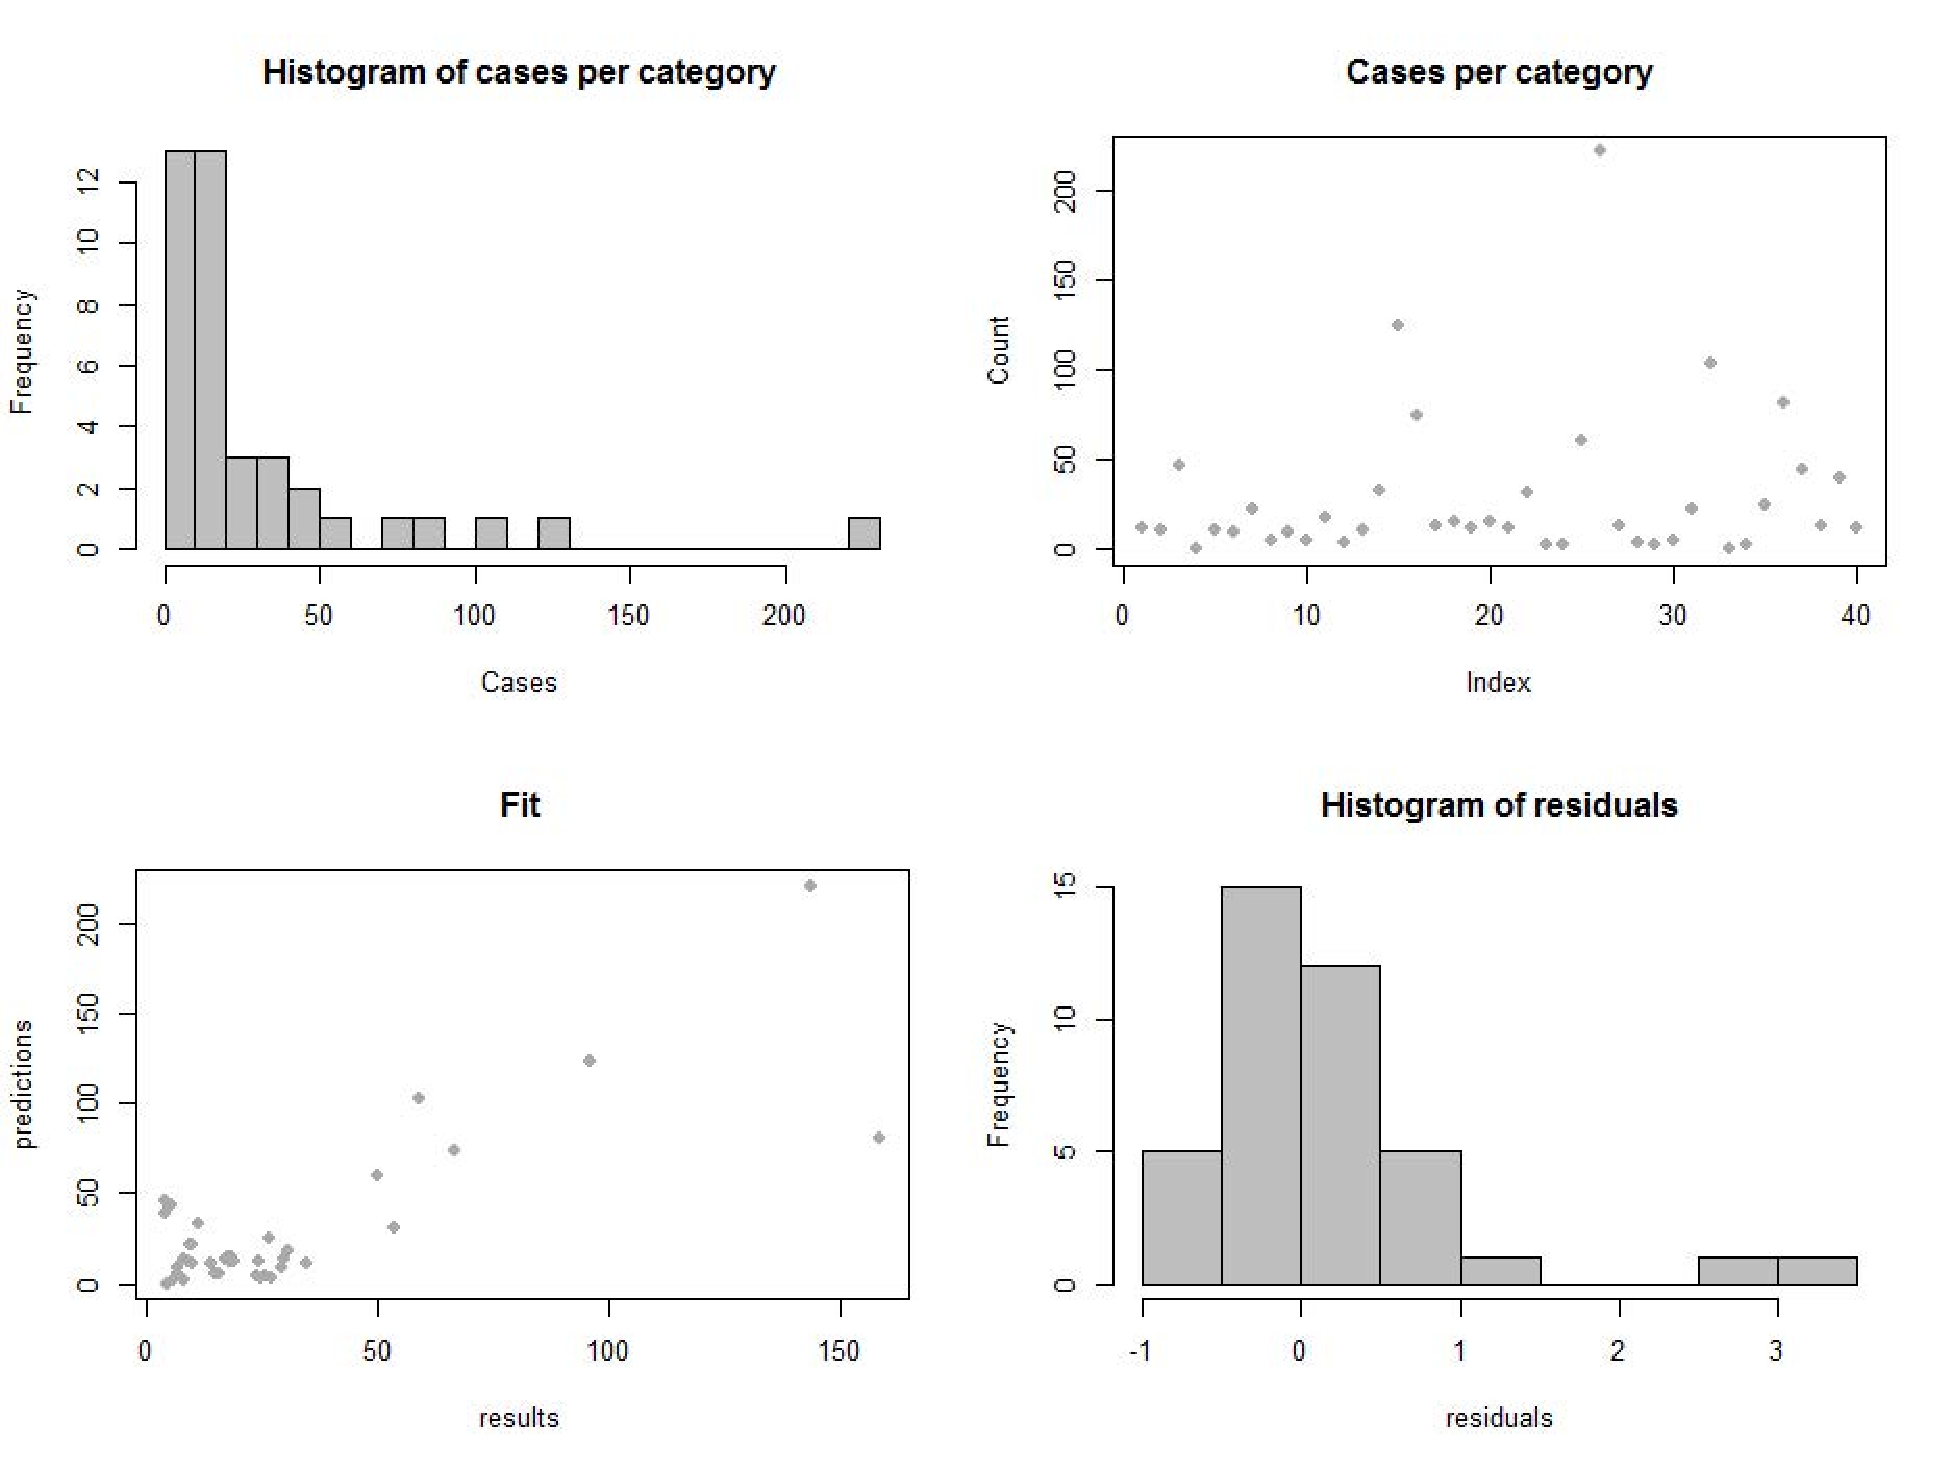
\includegraphics[width=0.9\textwidth]{Rplot_quasipoisson_noMLA.pdf}
     \caption{test}
     \label{fig:regn}
\end{figure}


\subsection{Risk analysis summary}
\begin{itemize}
\item There is a continued, and perhaps increasing, risk of measles importation due to travel and endemic measles elsewhere in the world.
\item There may be seasonal changes in risk of measles importation, though further analyses are needed.
\end{itemize}

\subsection{Future risk analyses}
We received the raw EpiSurv measles case data from The Institute of Environmental Science and Research Ltd (ESR) on 27 June 2014. Initial analyses of those data (not shown) suggest that we require denominator data to perform multivariate analyses to avoid confounding results due to a lack of independence among risk factors. Specifically for the multivariate analyses we wish to perform that detect interactions we require $\textsf{Age} \times \textsf{Prioritised Ethnicity} \times \textsf{NZDep}$ data for New Zealand to test whether interactions among case covariates provide additional information on risk over the univariate analyses performed in the report reviewed above. These $\textsf{Age} \times \textsf{Prioritised Ethnicity} \times \textsf{NZDep}$ data only became available to us on 3 July 2014, provided by the University of Otago.

The following analyses are in progress, for inclusion in later reports:
\begin{itemize}
\item Multivariate regression analyses to assess interactions between risk factors that may confound the univariate analyses.
\item Update of the importation risk analyses using a broader range of years, including modelling the trend in importations.
\end{itemize}
Additional data we believe would enable us and the Ministry to better understand measles risk is fine scale (lower than District Health Board (DHB)) immunisation coverage data. We understand the National Immunisation Register (NIR) allows tracking of the vaccination status of children and this is very useful, but inclusion of these data at lower (e.g. meshblock, census area unit) level would allow better understanding of risk of measles infection and resource allocation because they may allow targeted immunisation programmes. Thus the data gap that we have that will hinder us providing fine scale risk maps is:
\begin{itemize}
\item Meshblock (or census area unit) level immunisation coverage data to allow targeted immunisation and understanding of risk at a fine scale level.
\end {itemize}
An additional data set that would enable us to develop the understanding of measles importation risk is:
\begin {itemize}
\item The number of New Zealanders arriving from abroad each year, the countries to which they travelled, and length of travel.
\end{itemize}


\section{Modelling measles epidemics}
\label{sec:epidemic_modelling}

A previously-published model of the dynamics of measles infections in New Zealand has been used to evaluate the vaccination strategy in New Zealand of MMR1 at 15 months and MMR2 before 5 years \citep{roberts0,roberts4,tobias98}. The results show that achieving coverage of greater than 90\% at both vaccination opportunities is necessary if future epidemics of measles are to be prevented.

The original mathematical model for the dynamics of measles in New Zealand prepared in 1996 \citep{tobias98} successfully predicted the 1997 epidemic, which was curtailed by a mass vaccination campaign \citep{mansoor98,roberts0}. Subsequent extension of this work in 1998 showed that the then current schedule of MMR1 at 15 months and MMR2 at 11 years was insufficient to prevent further epidemics. The model developed by \citep{roberts0} supported the change in the immunisation schedule that took effect in January 2001, at which time MMR2 was changed from delivery at 11 years to delivery before the age of five. The schedule was changed in 2000 with MMR2 now being administered before 5 years \citep{anon2a} and later analyses suggested high levels of vaccination coverage (but less than 95\%) could eliminate measles, but emphasised that it is necessary to maintaining high coverage rates in order to prevent future epidemics \citep{roberts4}.

These results were comparable to others, for example: \citep{babad95} suggested two-dose schedule for England and Wales, with the second vaccination given at age four; and \citep{gay98} recommended a second vaccination at either 18 months or five years, to complement the first vaccination at 12 months in Canada. In addition, \citep{agur93} found that vaccinating 85\% of susceptible children aged one to seven years at five-yearly intervals would prevent epidemics in Israel. All agree that two vaccinations at no less than five years apart are necessary to prevent measles epidemics. \citep{wallinga1} took existing policies in eight European countries and estimated the coverage rates required to reduce $R_v$ below one. They found that results depended on the age at delivery, but no strategy succeeded if coverage rates were below approximately 87\%.

Numerous models for measles vaccination strategies for various regions \citep{agur93, babad95, edmunds0, gay98, wallinga1} based on sets of nonlinear differential equation (ODE) models have reached similar conclusions. The differences in the models have been in the details of the representation of the infectious period, and in the ways in which the age and contact structures of the population have been specified. While analyses suggest that 85\% coverage at MMR1 and MMR2 could be sufficient to prevent future measles epidemics, \citep{glass4} in the Netherlands showed that high overall levels of measles vaccination can obscure pockets of poor coverage, resulting in localised regions with increased risk of infection and effective immunisation is difficult to evaluate. 

The quantity that determines whether an epidemic will occur is the basic reproduction number of the infection, $R_0$. This is defined as the expected number of secondary infections that would arise from a single primary infection introduced into a fully susceptible population \citep{anderson91, diekmann0}. If $R_0 > 1$ an epidemic will occur following an introduction of infection. The best estimate for measles in New Zealand was $R_0$ = 12.8 \citep{roberts4}. The basic reproduction number of the infection under vaccination, $R_v$, is the expected number of secondary infections that would arise from a single primary infection introduced into a vaccinated population at equilibrium and is a robust indicator of the performance of a vaccination schedule. If $R_v < 1$ epidemics are prevented. The case reproduction number of the infection at time $t$, $R_t$, is the expected number of secondary infections that arise from a single infection at a particular time and depends on the number in the population who are susceptible.

\subsection{Modelling methods}

To understand the level of immunity in the population, the transmission dynamics of measles in the partially immune population and how likely an outbreak was of becoming endemic, we estimated $R_v$ from all the outbreaks in New Zealand since 2009. To do this we estimated $R_t$, following an adaptation of the methods in \citep{obidia12,wallinga4}. We were required to compute the generation time for measles to do so. The generation time is the average time an index case infects others after becoming infected. We used a lognormal distribution with mean 12.0 and standard deviation (s.d.) 3.5 from \citep{klinkenberg11}. We then estimated $R_t$ from the incidence data for each outbreak, defining outbreaks in the dataset given their temporal and geographic correlations (Figure~\ref{fig:dhbcases}). The outbreaks we used in our analyses are shown in Figure~\ref{fig:outbreaks}.

\begin{figure}
     \centering
     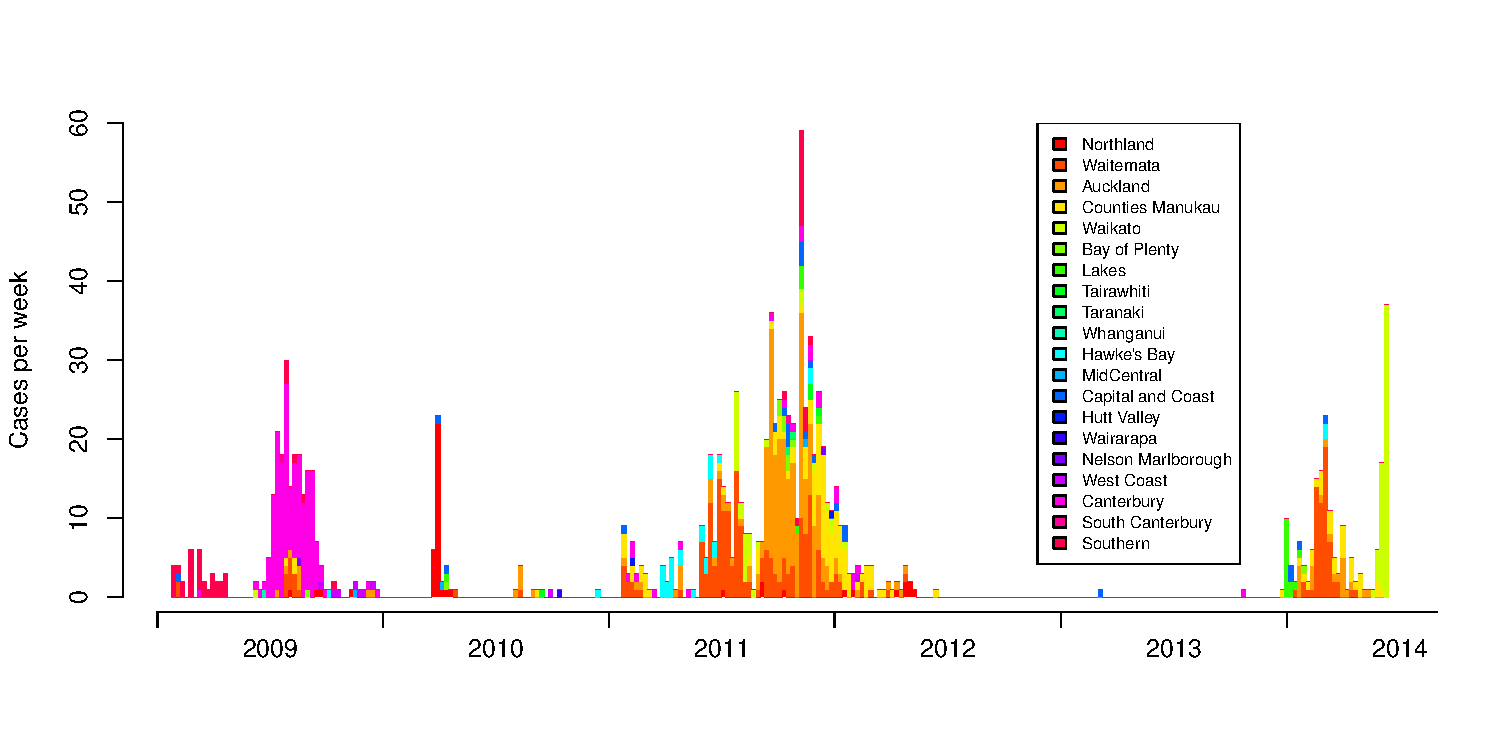
\includegraphics[width=0.9\textwidth]{cases_by_dhb_2009_2014.pdf}
     \caption{Measles cases by district health board (DHB) from 2009 to 2014}
     \label{fig:dhbcases}
\end{figure}

\begin{figure}
     \centering
     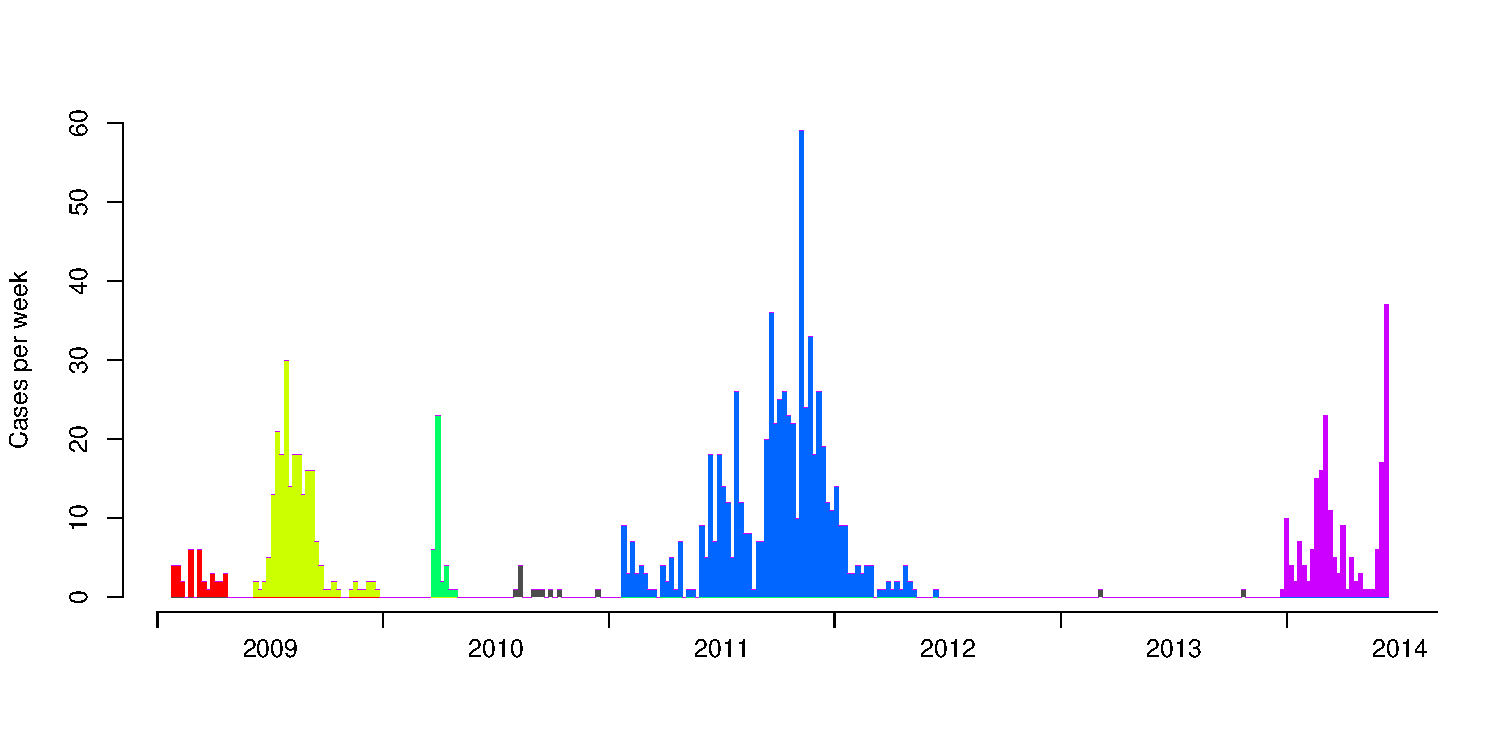
\includegraphics[width=0.9\textwidth]{outbreaks_for_R0.pdf}
     \caption{Measles data classified as outbreaks for reproductive number of the infection ($R_v$) estimation}
     \label{fig:outbreaks}
\end{figure}

\begin{figure}
     \centering
     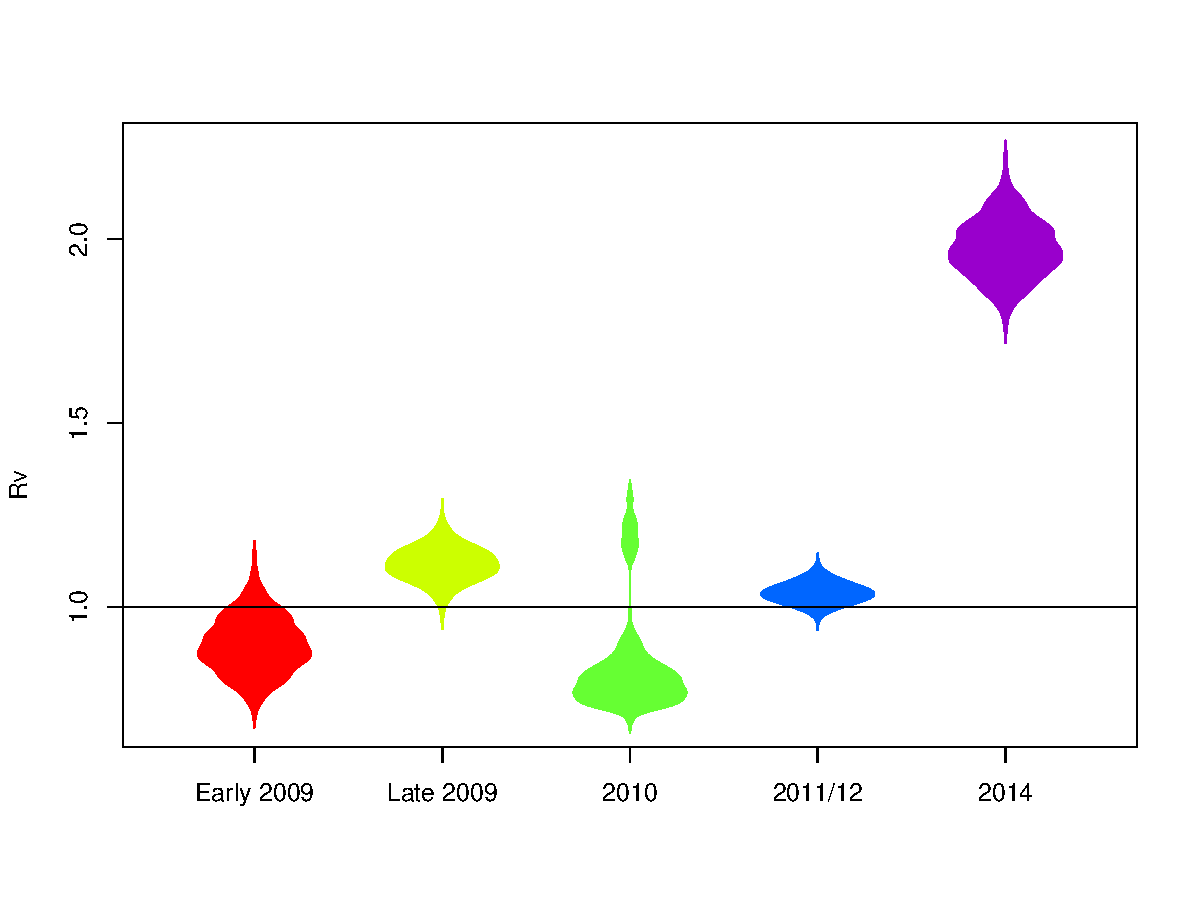
\includegraphics[width=0.9\textwidth]{averageR0.pdf}
     \caption{Estimates of $R_v$ ($R_0$) for the outbreaks each year, as classified in Figure~\ref{fig:outbreaks} (page~\pageref{fig:outbreaks})}
     \label{fig:r0}
\end{figure}

\begin{figure}
     \centering
     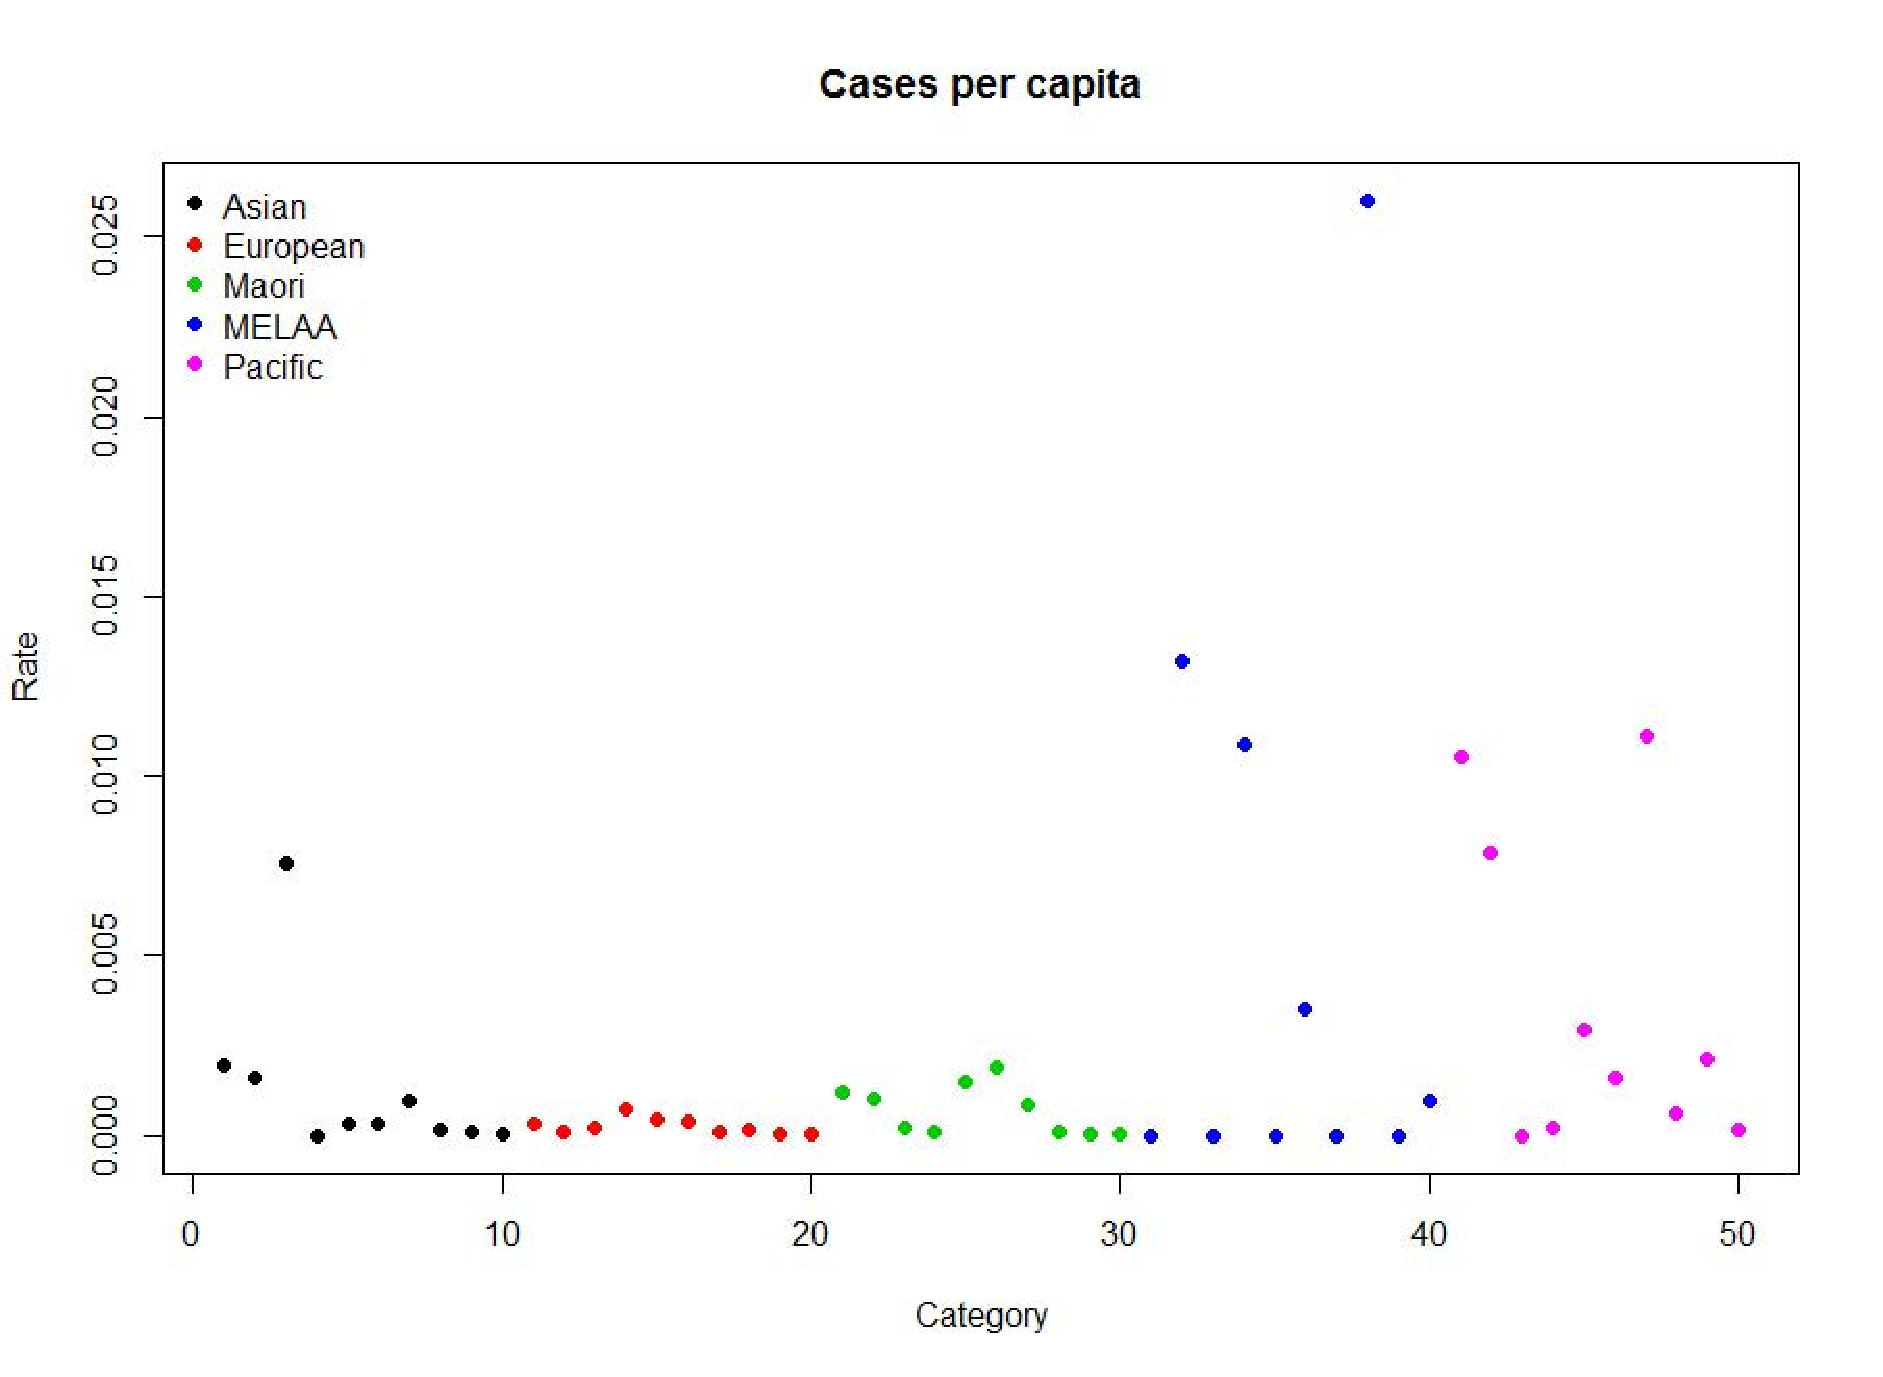
\includegraphics[width=0.9\textwidth]{PerCapitaCases.pdf}
     \caption{test}
     \label{fig:percap}
\end{figure}

\begin{figure}
     \centering
     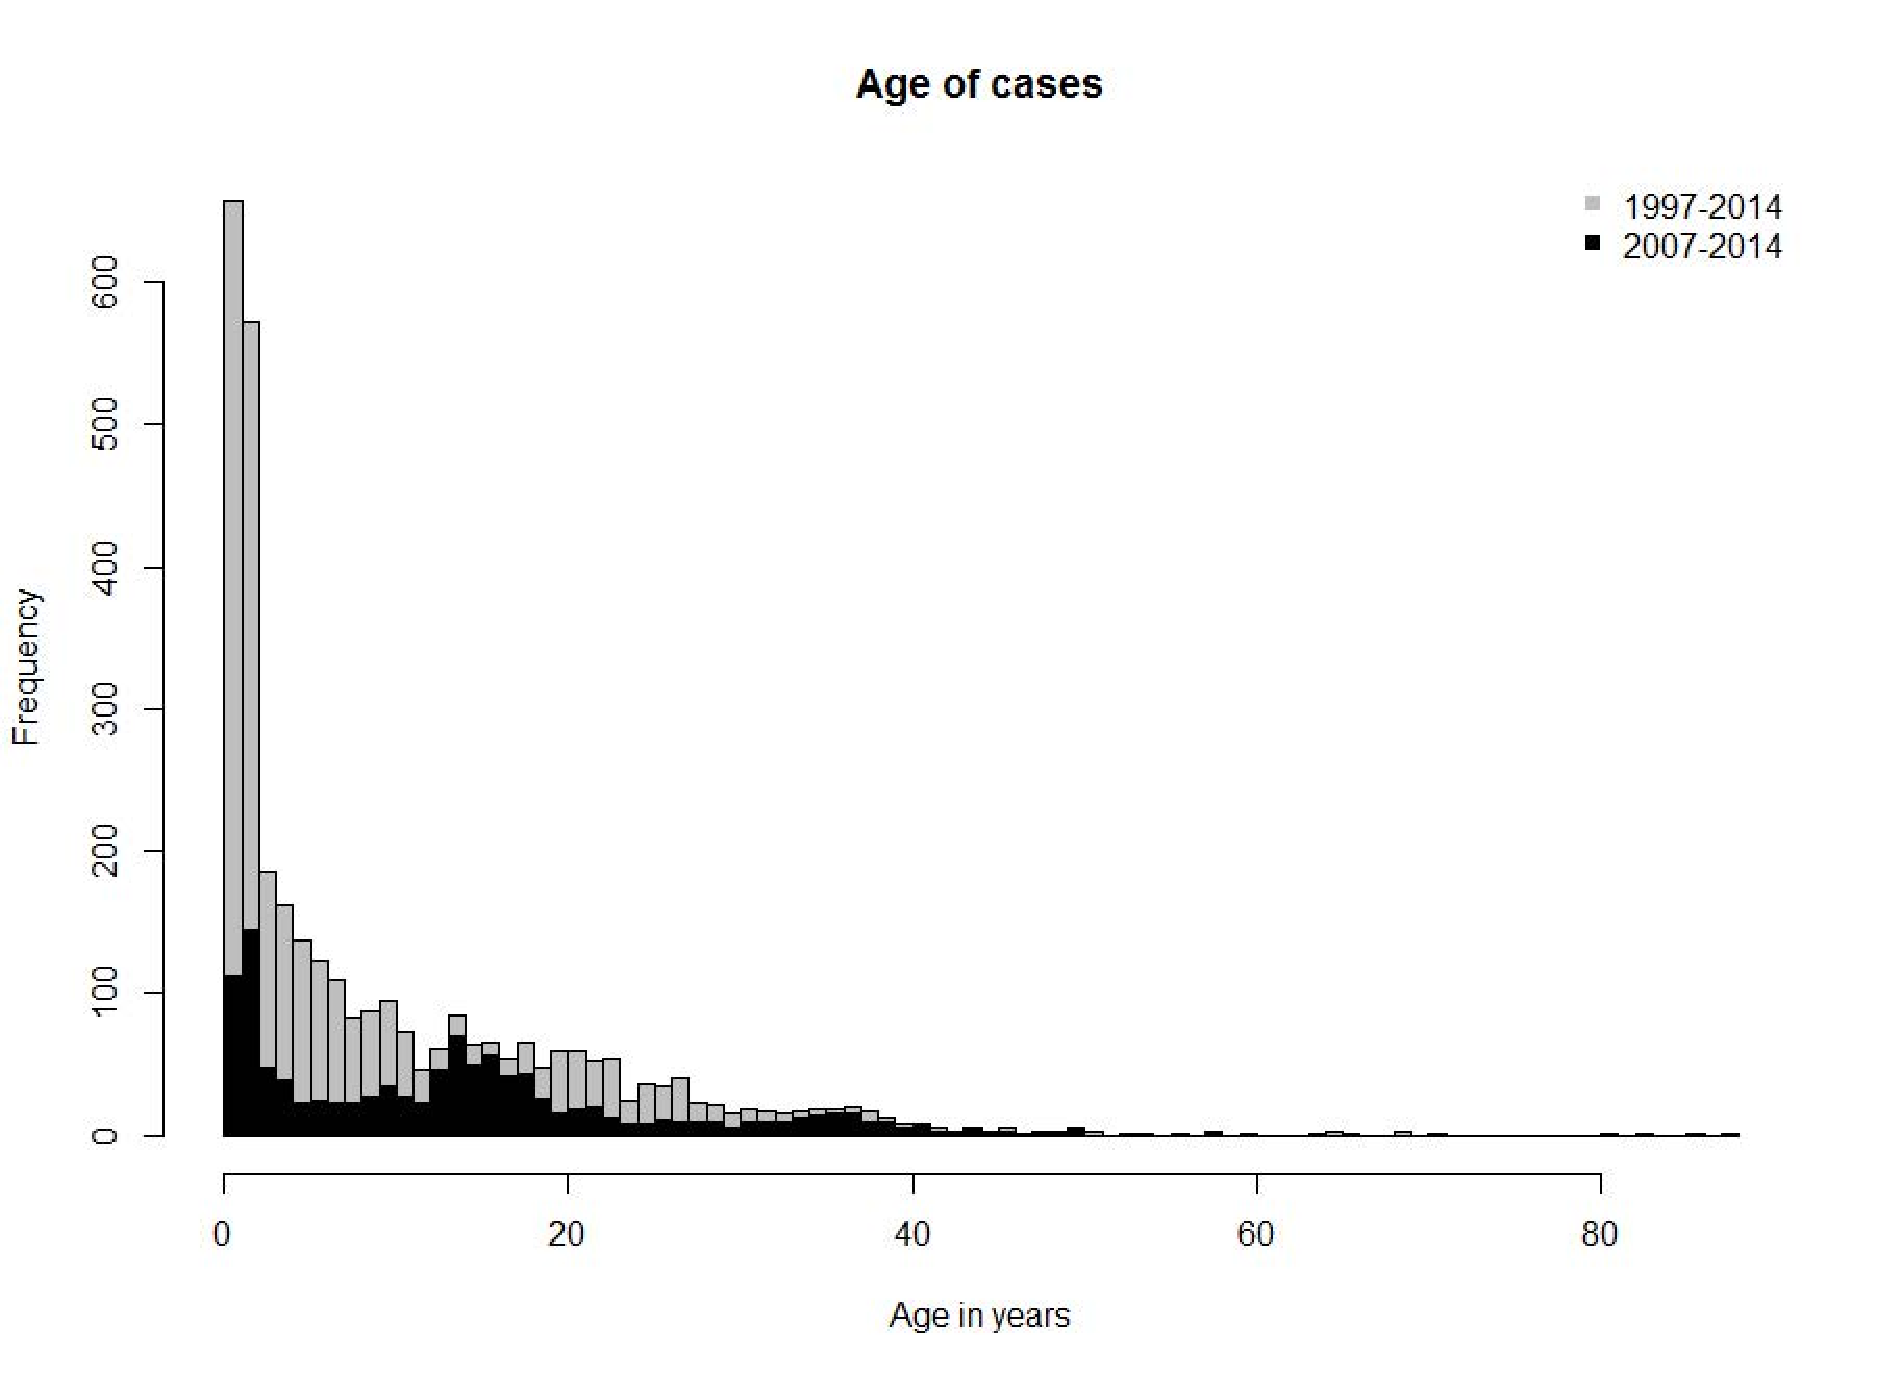
\includegraphics[width=0.9\textwidth]{AgeCases.pdf}
     \caption{test}
     \label{fig:agecases}
\end{figure}

\begin{figure}
     \centering
     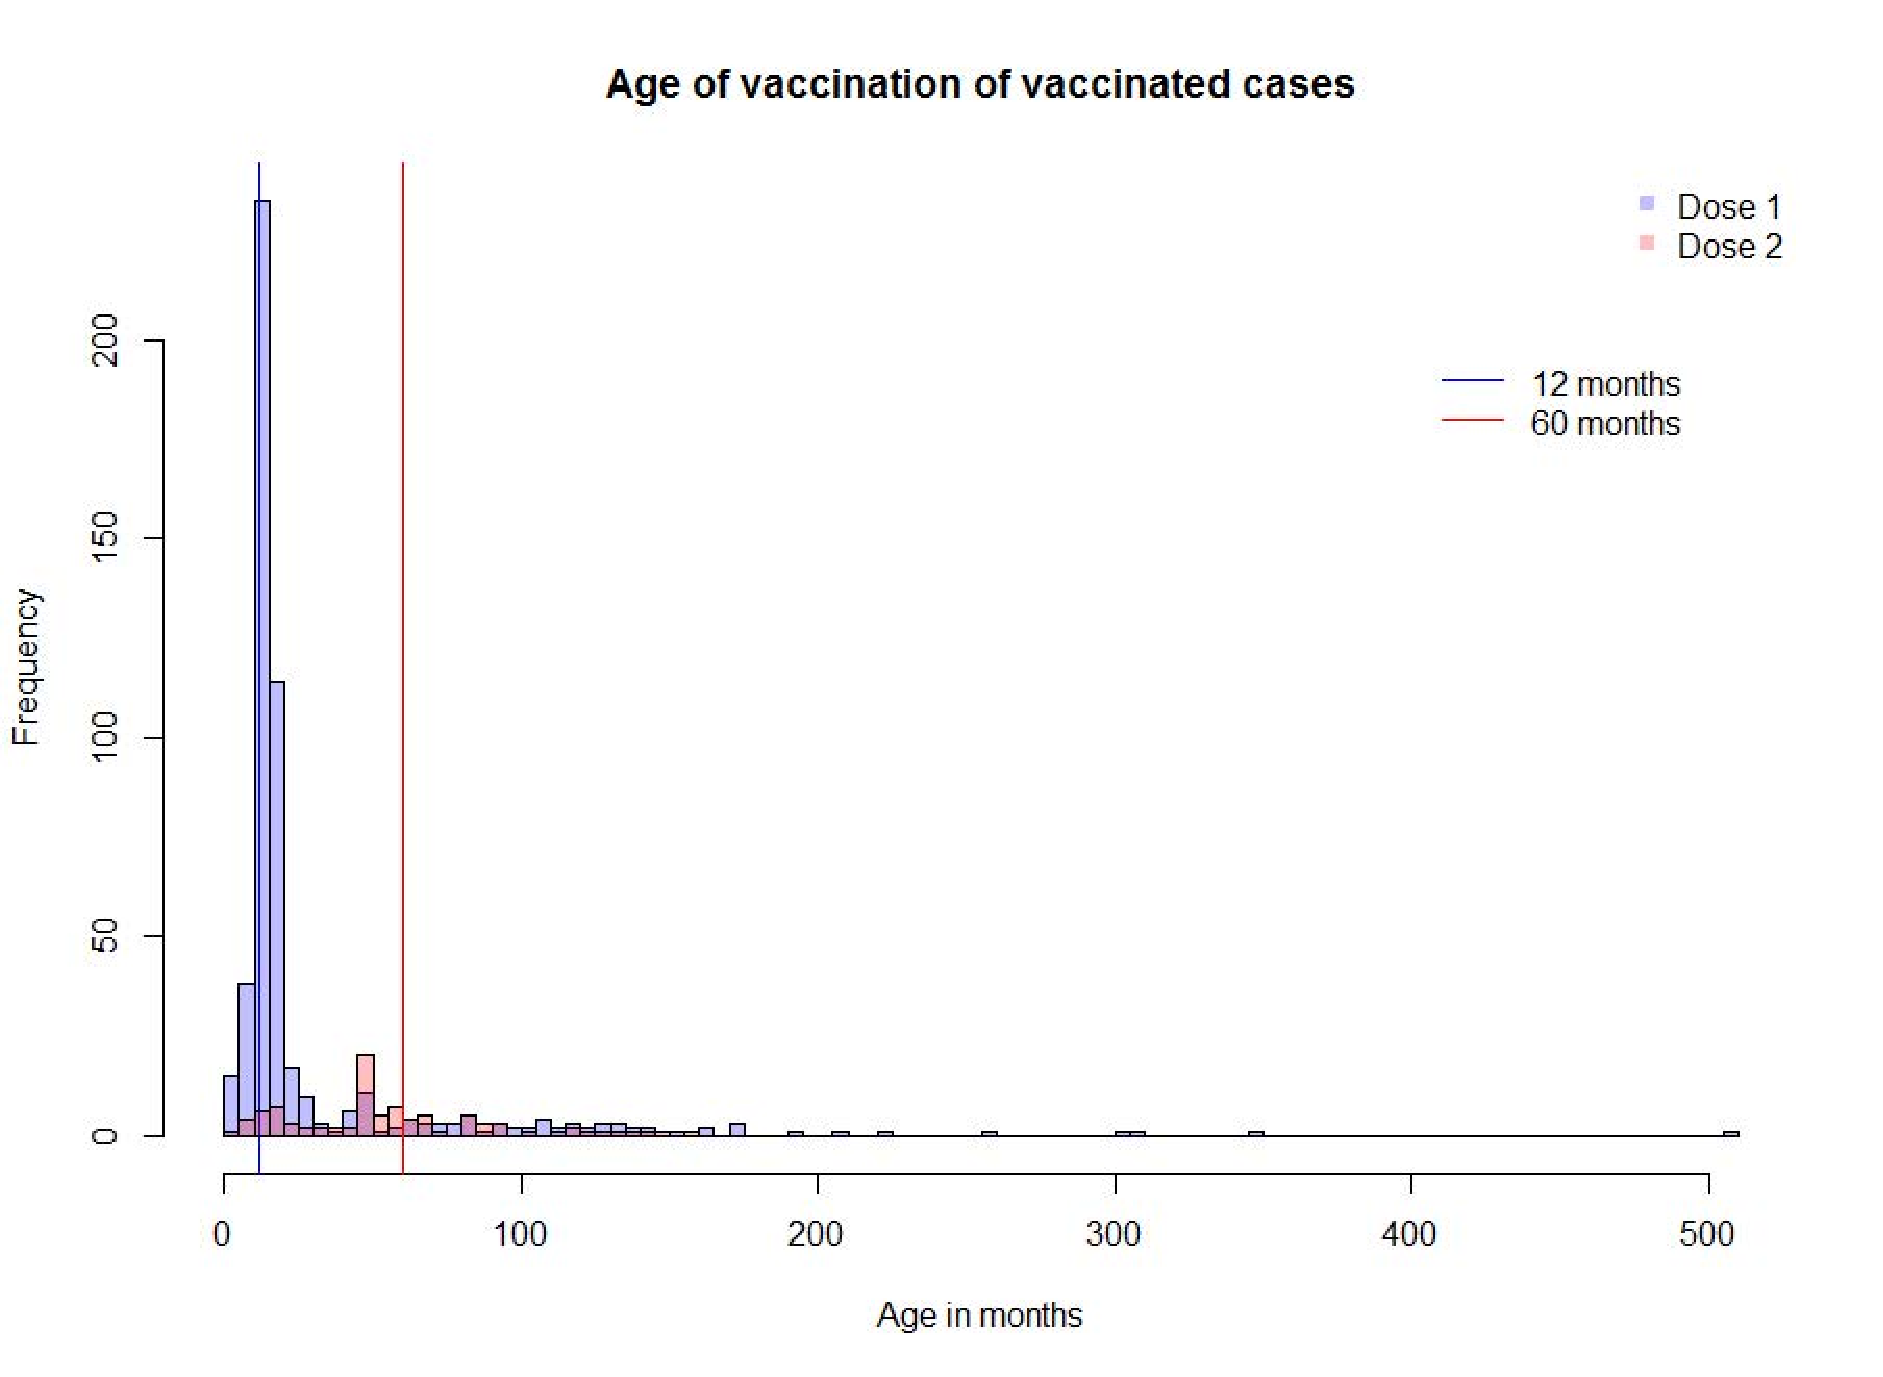
\includegraphics[width=0.9\textwidth]{AgeOfVaccinationVaccinated.pdf}
     \caption{test}
     \label{fig:ageofvacc}
\end{figure}

\begin{figure}
     \centering
     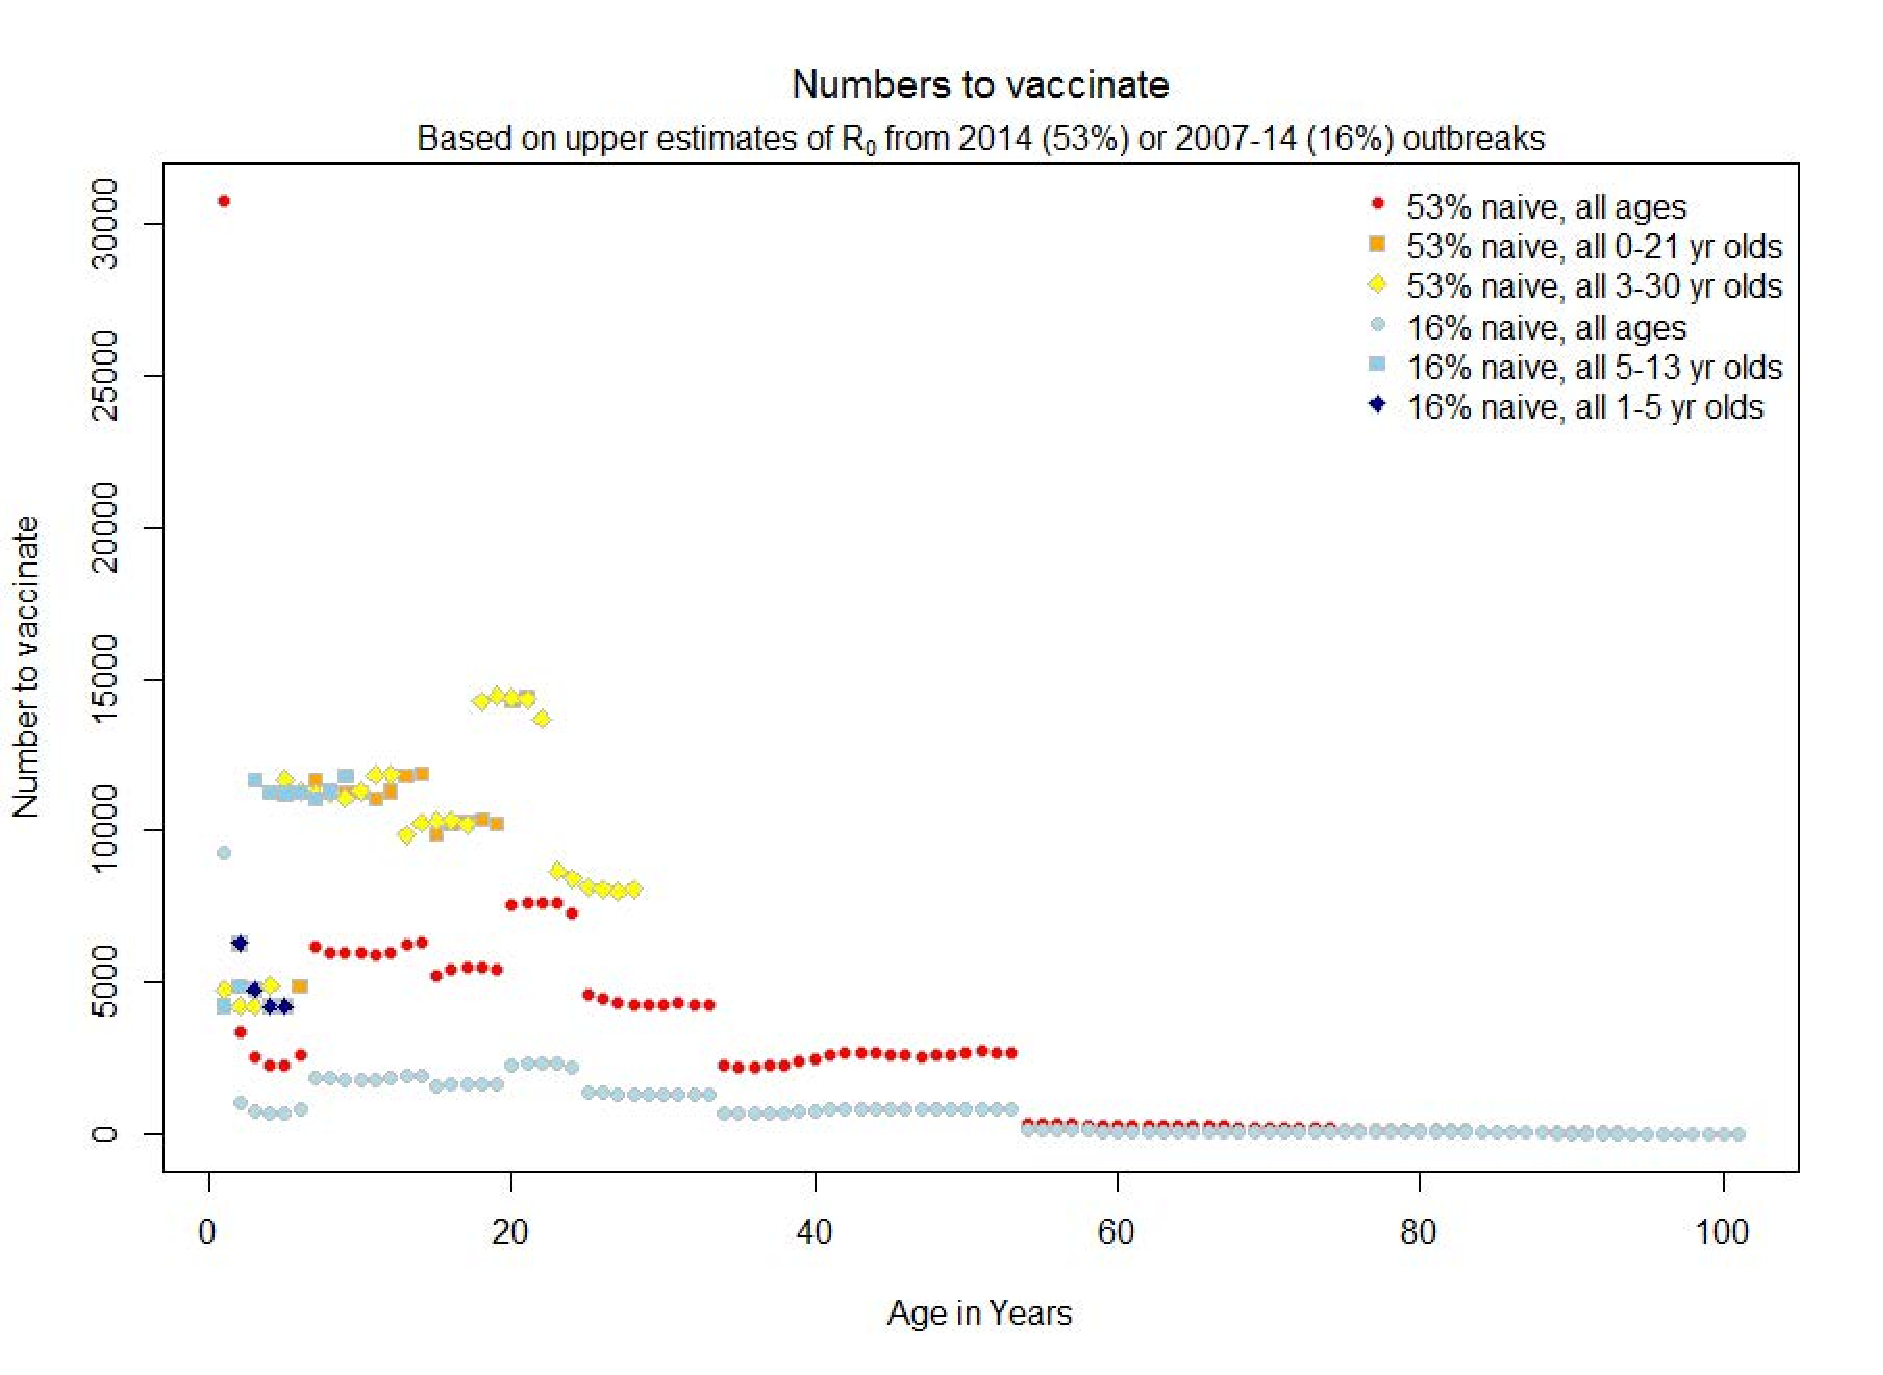
\includegraphics[width=0.9\textwidth]{NumbersToVaccinate.pdf}
     \caption{test}
     \label{fig:numvacc}
\end{figure}

\begin{figure}
     \centering
     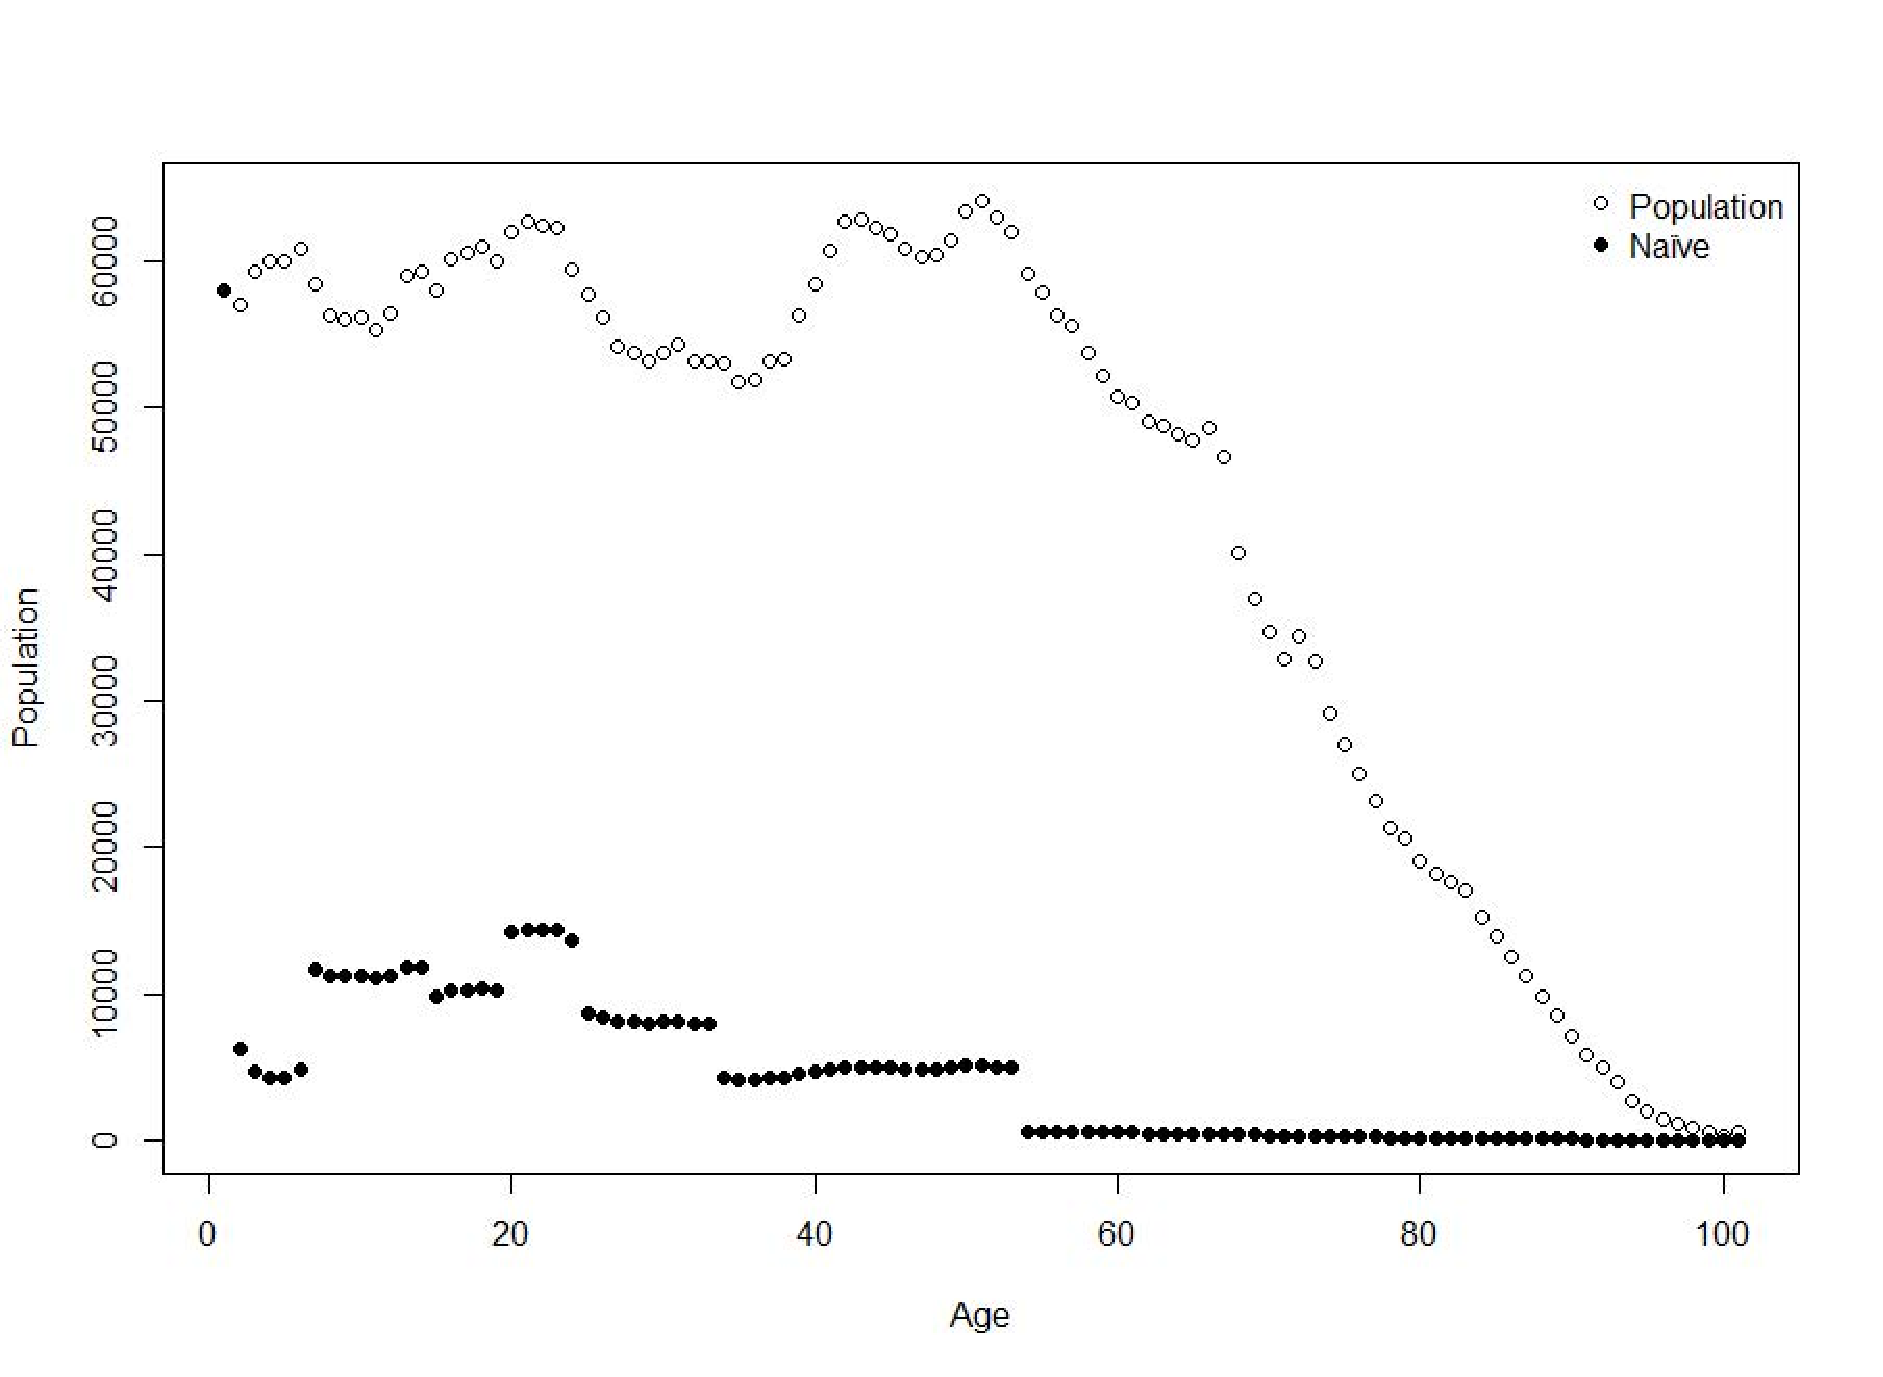
\includegraphics[width=0.9\textwidth]{PopulationNaive.pdf}
     \caption{test}
     \label{fig:naive}
\end{figure}

\begin{figure}
     \centering
     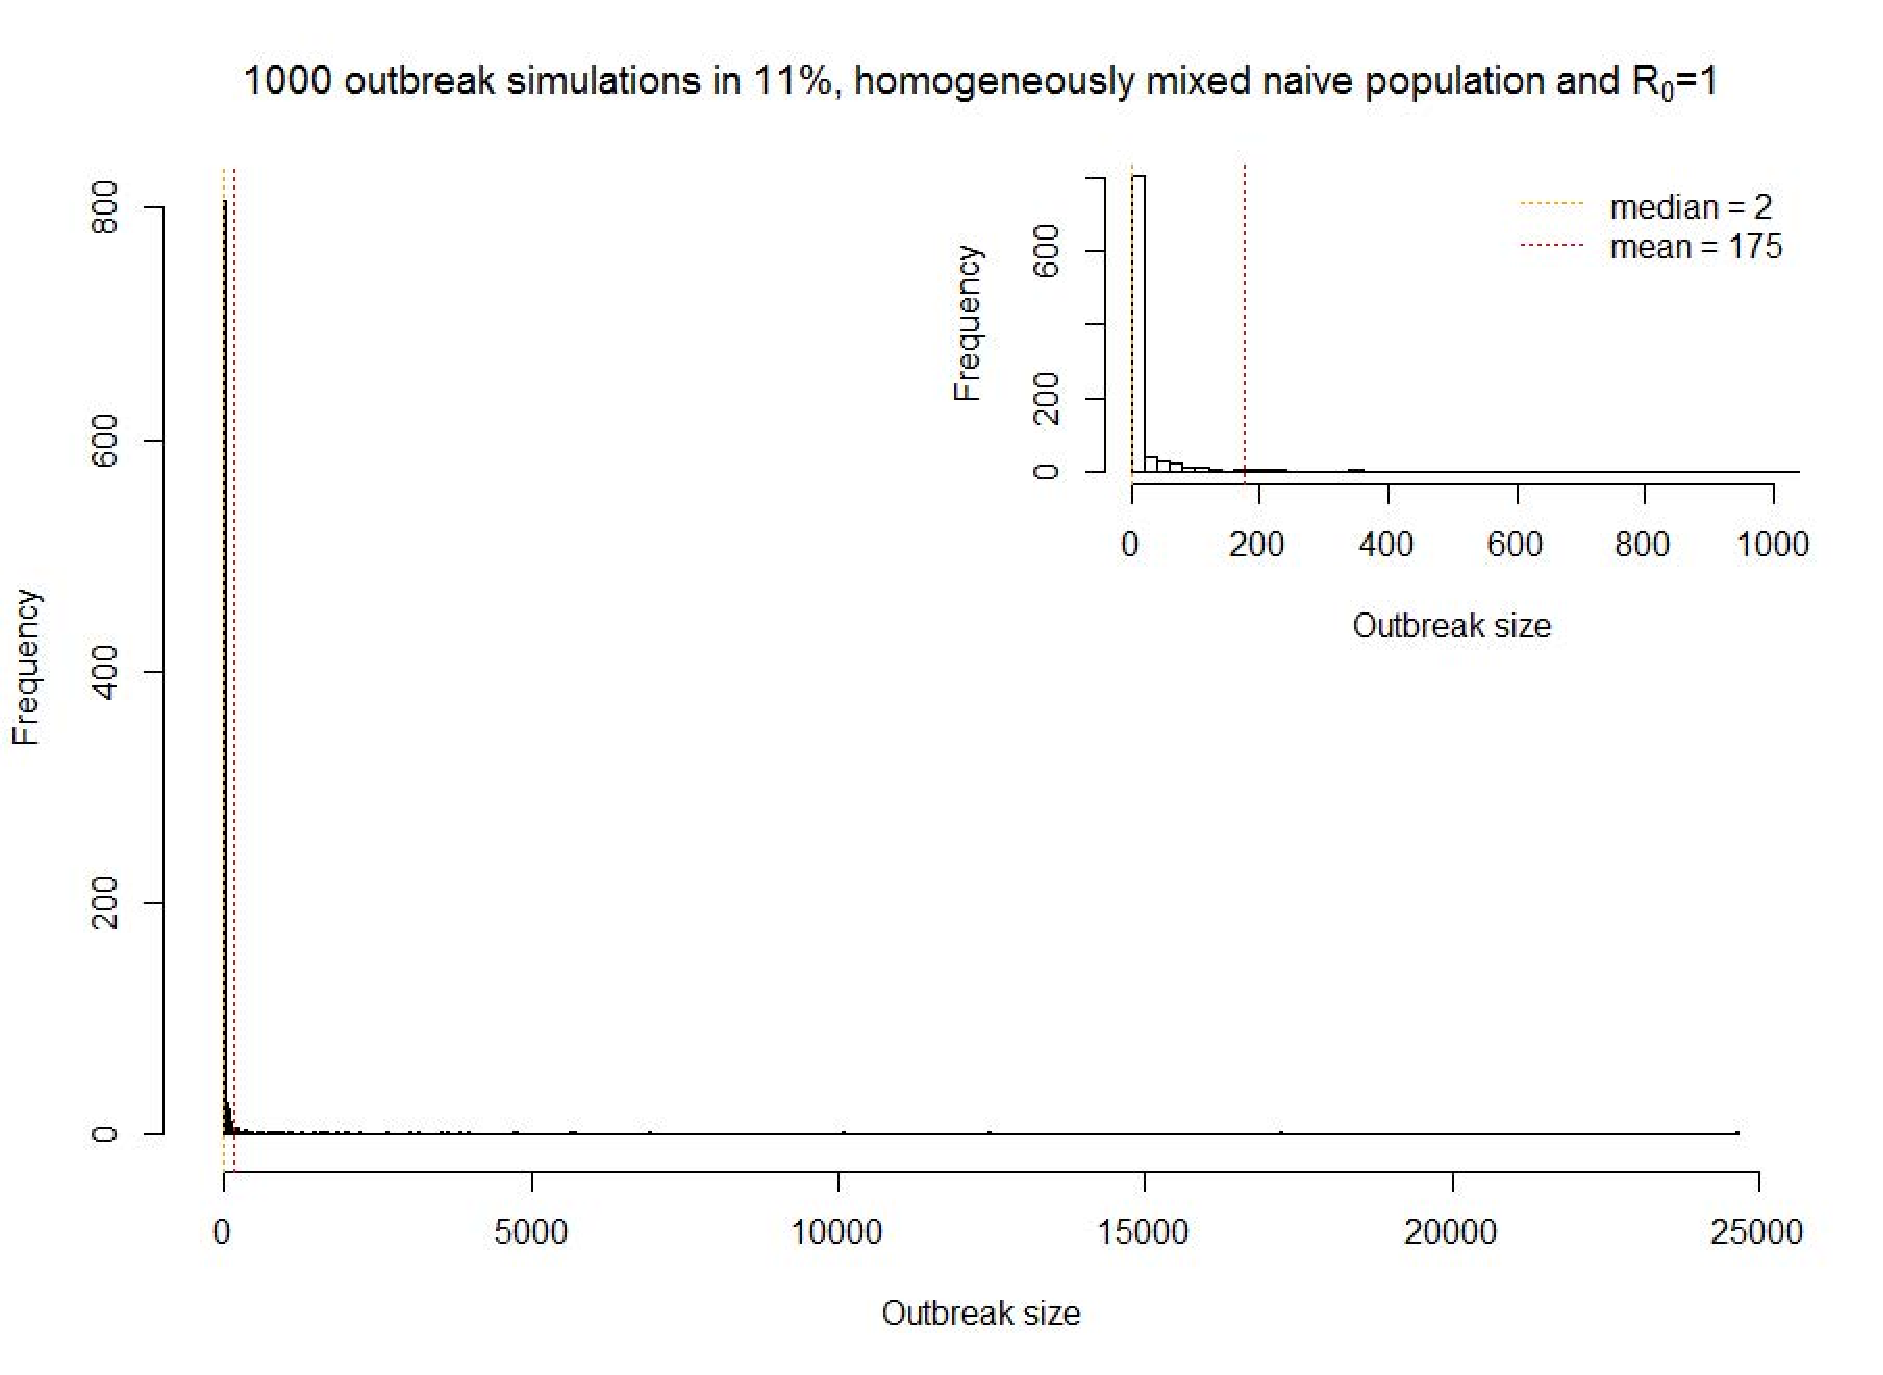
\includegraphics[width=0.9\textwidth]{simulations.pdf}
     \caption{test}
     \label{fig:sim}
\end{figure}

\begin{figure}
     \centering
     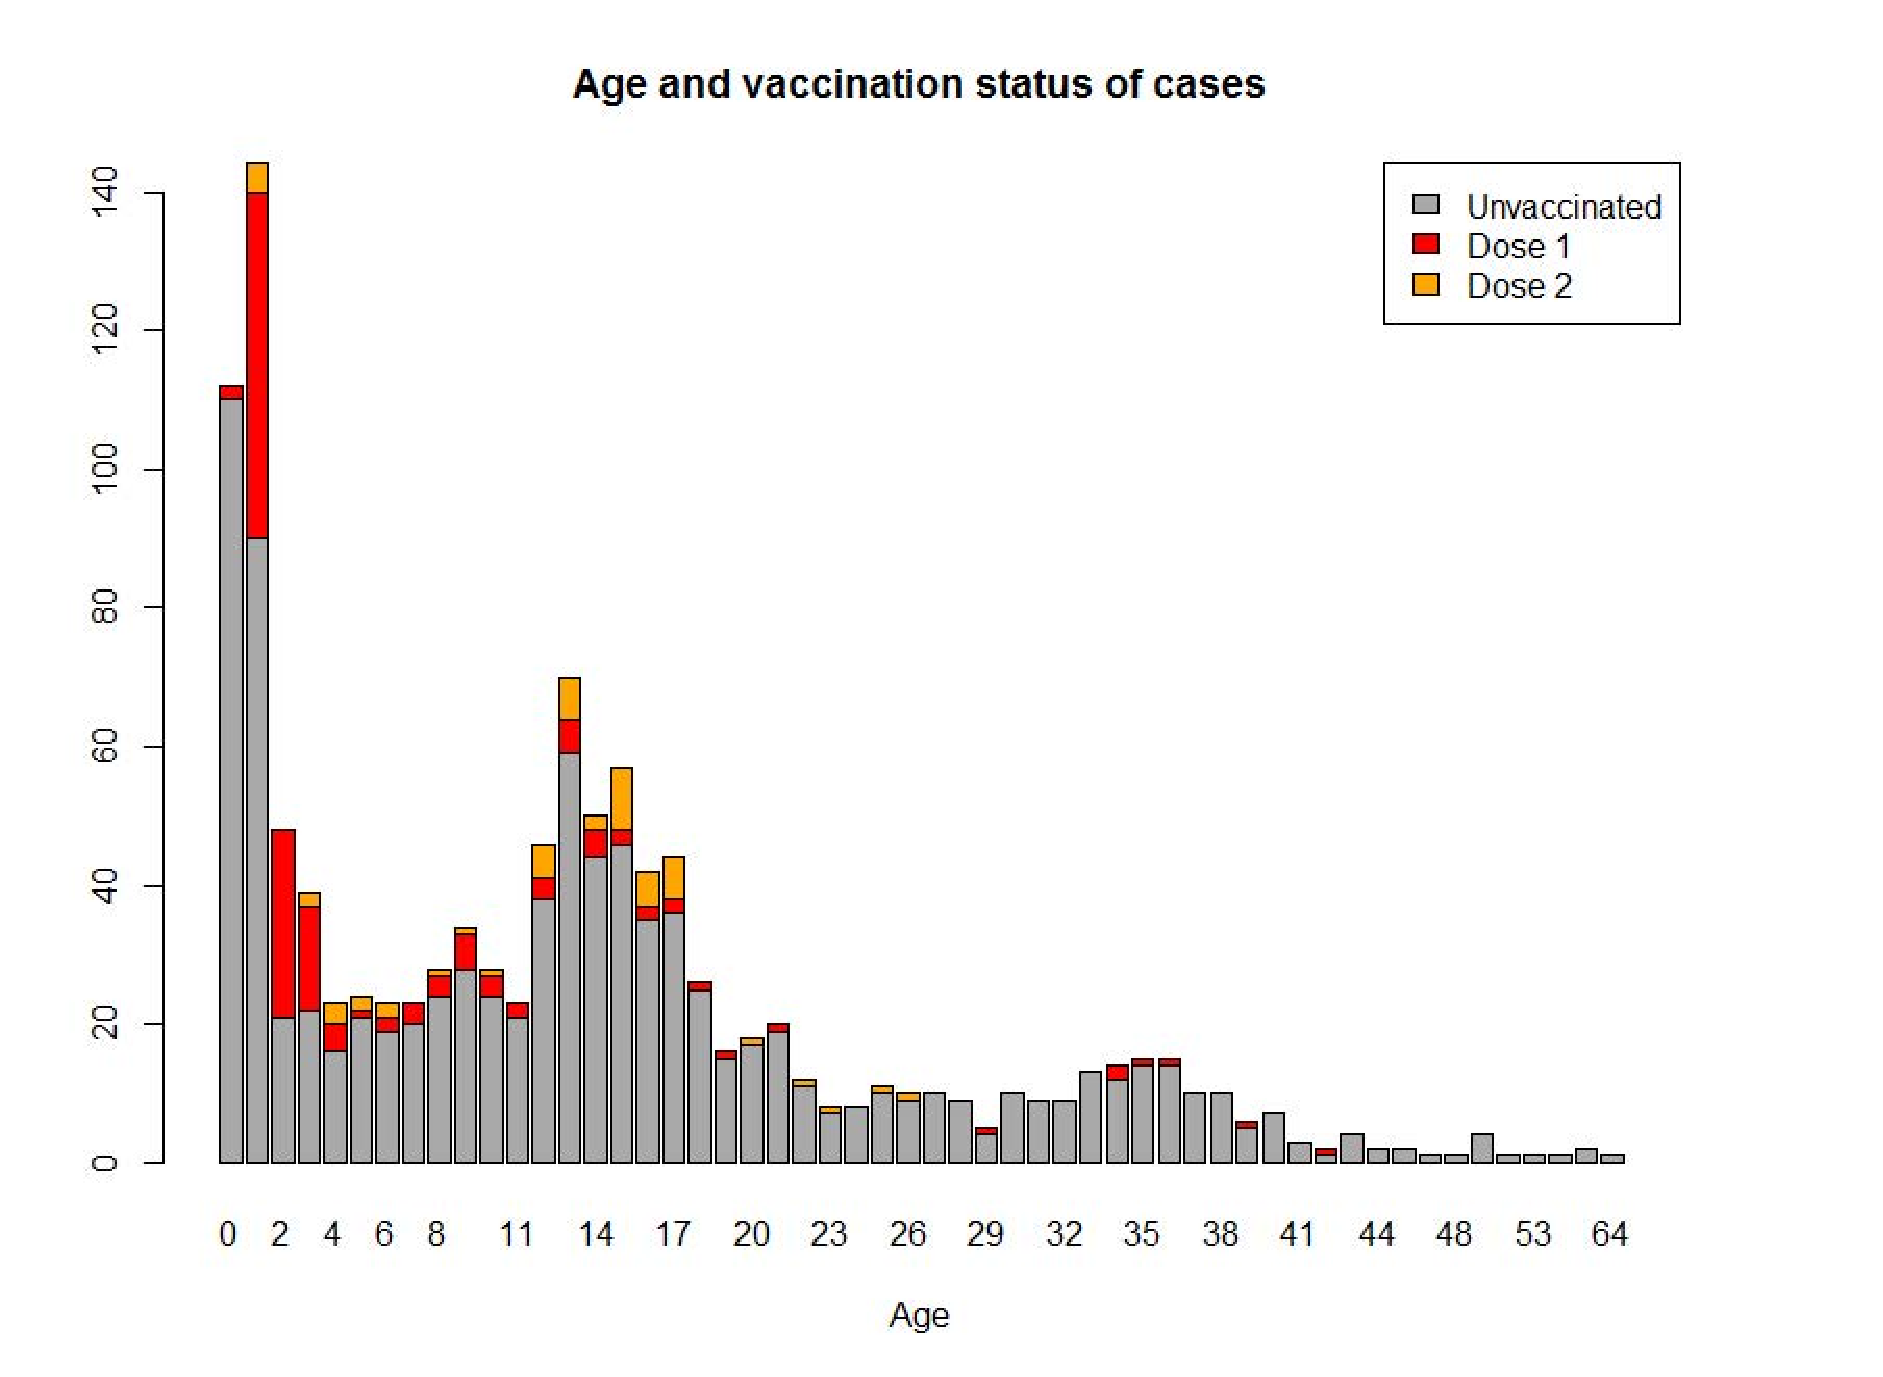
\includegraphics[width=0.9\textwidth]{vaccinationstatusage.pdf}
     \caption{test}
     \label{fig:vaccstat}
\end{figure}


\subsection{Modelling results and discussion}

The estimated $R_v$ for each outbreak is shown in Figure~\ref{fig:r0}. The probability density of the $R_v$ estimates for each outbreak all include one. Of particular note is the ongoing outbreak, which has an $R_v$ well above one and thus we may expect this outbreak to persist if conditions remain the same. An important caveat to this outbreak analysis is that because this 2013--2014 outbreak is an ongoing outbreak, and not in decline, $R_0$ is necessarily over one, and so the comparison with others must be cautious.

These analyses also imply that the regular (approximately yearly) importation of measles is an ongoing process. Given the risk of importation of measles as highlighted in section~\ref{sub:risk_analyses} is likely to continue, these analyses suggest substantial efforts are required to maintain the level of immunisation to high enough levels that measles does not become endemic. The measles outbreak in 2011--2012 had an $R_v$ of just greater than one, and yet it persisted for over 12 months. This implies that the current outbreak may persist within the population for a substantial period, given it's $R_v$ is approximately twice that of the 2011-2012 outbreak. A caveat to this and other $R_v$ estimates is that the 2013--2014 outbreak may include some sporadic cases and thus the true basic reproductive numbers may be lower than estimated. However, sub-clinical and underreporting may lower the estimate. The relative contributions of both to our estimates are currently unknown.

\subsection{Summary of modelling}
\begin{itemize}
\item Regular introductions of measles pose an ongoing threat to New Zealand's efforts to eliminate measles (also see section~\ref{sub:risk_analyses}).
\item The reproduction number for measles in a partially immune population is often close to one, suggesting increased population level immunity is required to prevent this measles persisting.
 \item The reproduction number, $R_v$, for measles in the current outbreak is well over one, suggesting that this outbreak has the potential to persist for prolonged periods, with the caveat that this estimate was made during the ongoing outbreak.
\end{itemize}

\subsection{Future modelling}
Future modelling we aim to perform are:
\begin{itemize}
\item An update of previous ODE models of measles in the overall population according the differing vaccine coverage scenarios \citep{roberts4}.
\item Model measles outbreaks with differing scenarios of measles importation into various population groups based on current introduction rates.
\end{itemize}


\section{Cost analyses}

In this section we provide a review of the costs of measles from other locations and an analysis of the costs involved with the current measles outbreak.

Approximately 50 years ago, approximately 135 million cases and 7--8 million deaths were believed to occur in the world due to measles \citep{clements4}. Thirty years later, it was estimated there were still approximately 45 million cases of measles occurring annually, including 6 million measles-related fatalities. \citep{wolfson7} estimated that in 1999 measles was responsible for more than 30 million disability adjusted life years (DALYs) lost and 12 million in 2005. Similarly, the number of cases was reduced by more than 50\% from 43 million in 1999 to approximately 20 million in 2005. They estimated approximately 7.5 million deaths from measles were avoided from 2000--05 due vaccination. The World Health Organization (WHO) estimated 158,000 deaths from approximately 355,000 measles cases in 2011 \citep{who13}.  In addition to the substantial losses occurring in measles-endemic countries, a significant impact is felt in heavily measles-vaccinated countries, which may be considered measles-free, due to contact with cases either in the country of origin or in the previously measles-free country.

The annual cost of treating and controlling measles in 11 industrialised countries was estimated to cost more than US\$150 million \citep{carabin3}. The estimated cost for a case ranged from US\$189--344 \citep{carabin3}; however, the average estimated cost of a typical hospital case ranges from US\$967--1,755 \citep{carabin2}. \citep{stack11} estimated the economic benefits from cases averted due to measles vaccination. They estimated that the expanded vaccination from 2005 to 2015 in 72 of the world's poorest countries could result in nearly US\$10 billion of costs averted between 2011 and 2020. Ninety-nine percent of these averted costs were the result of lost productivity due to an estimated 360,000 measles-specific premature mortalities, with the remaining <1\% associated with averted treatment costs and reduced caretaker productivity for the nearly 12 million measles cases avoided.

Italy has the highest reported annual cost of measles among industrialised countries \citep{carabin3}. In 2001, it reported losses related to measles of approximately US\$50 million. The economic impact of a large measles outbreak in Italy, 2002--03 examined the costs associated with 5,154 hospitalisations where measles was the main discharge diagnosis. The mean length of hospital stay was 5.2 days (median = 4 days and range = 1 to 303 days). The total cost of these hospitalisations amounted to \euro 8.83 million (\euro 1 $\approx$ NZ\$2.0 in 2002-03), or approximately \euro 1,700 per case. The average cost per non-complicated measles case was  \euro 1,429, while the mean cost of a case with complicated measles was  \euro 2,721. The average daily cost of a hospital stay was  \euro 327.

An outbreak of measles occurred in Sydney, Australia, lasting nearly 2 months in 2011 and resulted in 26 confirmed cases \citep{flego13}. Seven (27\%) of the cases required hospitalisation for more than 1 day and 10 (38\%) resulted in management within a hospital emergency department. During this outbreak, a total of 1,395 contacts were identified and managed by a public health unit in western Sydney. The mean number of contacts per case was 54 (median = 28, maximum = 206). The estimated cost to the public health unit for contact management for the epidemic was in excess of AUS\$48,000, with 90\% of this being associated with staff time. 

Germany implemented a two-dose measles vaccination program in 1991 and has seen the benefits in recent years. In 2001 more than 6,000 cases were reported in Germany but by 2004 this number fell to 122 \citep{wichmann9}. However, in 2005 more than 500 cases were reported by the middle of the year in two German states, with the vast majority (>95\%) in non-vaccinated children \citep{siedler6}. An economic analysis was performed of the 614 measles cases reported in an 8-month period in Duisburg in the state of North Rhine-Wesphalia (NRW). In that study, they estimated the health-care provider costs to be approximately \euro 229,000, or \euro 373 per case. Approximately 78\% of these costs were associated with the 95 (15.5\%) of the cases that were hospitalised. The mean costs of the hospitalised patients was  \euro 1,877, including one patient with encephalitis at a cost of \euro 35,623. In addition to the health-care provider costs, additional costs of \euro 89,400 were incurred by the district public health office, the majority (\euro 85,000, 95.1\%) for personnel, \euro 2,300 (2.6\%) for vaccination, and \euro 2,100 (2.3\%) for serologic testing. Therefore the combined direct costs of these 612 cases amounted to \euro 318,400, or \euro 520 per case. In addition, to determine the total impact, it would be necessary to include the indirect losses associated with lost production of cases and care givers.

Although measles was declared eliminated from the United States in 2000, it remains a concern due to the endemic nature of it around the world \citep{parker6}. Several studies have been conducted in the United States to assess the economic impact of recent measles outbreaks due to imported measles.  \citep{ortegasanchez14} estimated the economic impact to public health departments in the US as the result of 16 outbreaks in 2011. The outbreaks lasted an average of 22 days and resulted in 107 confirmed cases; however, from these 107 cases, they estimated between approximately 8,900 and 17,500 contacts with confirmed cases, requiring between 42,600 and 83,100 personnel hours at a cost of between US\$2.7 and 5.3 million. Overall, it was estimated that each contact required 4.7 personnel hours at a cost of US\$298 per contact.
\citep{dayan5} calculated the cost of containing a single case of measles that occurred in Iowa in 2004. They estimated that for the one week that the Iowa Department of Public Health (DPH) investigated the case, 2,525 hours were used to identify contacts, set up vaccination clinics, and institute and enforce quarantine orders for those who refused vaccination. In total, it was estimated the direct costs associated with three cases of measles was US\$142,452, or nearly US\$50,000 per case.

\citep{parker6} reported the impact of a large measles outbreak due to a non-autochthonous case in Indiana. A total of 34 cases, 94\% of which were not vaccinated against measles were reported in the outbreak. Direct cost information was obtained from approximately 100 public health officers and infection-control officials needed to control the outbreak. Direct cost for those completing a survey showed the outbreak cost at least \$167,685, 83\% of which (\$139,023) was for wages, salaries and overhead. This amounted to a direct cost of \$4,932 per measles case. These costs did not include either patient care or indirect costs, which would have made the total and per case cost higher.

\citep{coleman12} estimated the direct medical and public health costs in response to a single case of refugee-imported measles.  Costs included labor, translation and benefits for public health workers. In addition, medical costs were incurred due to vaccination, immunoglobulin, testing for measles immunity, hospitalisation, transportation and diagnosis. In total, 387 hours were associated with this single case, resulting in a cost of US\$11,881. In addition, per-contact costs amounted to US\$264. The cost of hospitalisation for the 3-day stay by the index case was US\$931. Additional costs were associated with physician visits (US\$294), vaccine and immunoglobulin (US\$1,765), mileage (US\$205) and immunologic screening tests for the parents' exposed to measles (US\$240) for a total of US\$23,816.

Economic analyses of measles control programs have shown them to be financially effective. In the Republic of Korea, the economics of alternative measles vaccination programs were compared. All of the alternatives were found to be economically efficient (benefit/cost ratio (B/C) > 1.0), with the alternative using two doses of the MMR program, with a catch-up campaign for measles and rubella being the most favourable (B/C = 1.27).

The purpose of the current study is to estimate the cost of the current measles outbreak in New Zealand. Using this information, we will then evaluate the economics of alternative measles control strategies in order to provide additional information to public health officials and decision makers.

.....Since 2009, all the outbreaks in New Zealand were linked to infections acquired (imported) from overseas, though previous work suggests these outbreaks still largely affect school-aged children and children under two years of age. Under two year olds are thought be be consistently among the most affected age groups because the first of two doses of measles, mumps and rubella vaccine (MMR) is not due until fifteen months.....

\subsection{Cost analyses methods}
Costs were evaluated as either direct or indirect. Direct costs included physician consultations, hospitalisations, drugs, vaccination, long-term care for chronic sequelae, special education costs. Direct costs can be divided into medical and non-medical \citep{saha13}. Direct medical costs include costs for diagnosis, treatment, continuing care, rehabilitation and terminal care. Personnel time (investigation and emergency response), materials (phone calls, vaccine), personnel (cost, wages and fringe benefits), overhead costs, public information, and mileage are estimated when calculating direct medical costs. Direct non-medical costs include transportation to and from health care providers.

Indirect costs are productivity losses for the case and/or health care provider, e.g. parent of a school child. Indirect costs included work loss for cases and caregivers. This could also include the economic value of premature life lost, costs associated with permanent disability, e.g. deafness and mental retardation. Commonly the human value approach (HVA) has been used to estimate economic impact of life. The HVA measures the potential future earnings of an individual and discounts it into a present value. Typically this is 3\% but 5\% has also been used in a sensitivity analysis, which is more compared to non-human life calculations and will tend to reduce the present value of the future earnings (saved by avoiding a case).

Data for the current measles outbreak were obtained from the New Zealand Ministry of Health, from 2008 through June 2014. Data included information on gender of the case, ethnicity and age of the case at discharge from hospital, days spent in the hospital, year of case, number of events, case weight and associated cost.

Cost of the Auckland Regional Public Health Service (ARPHS) for measles response were obtained from the Ministry of Health. Data, for the period January 1 - March 9, 2014, reported salaries for people involved with the measles outbreak management medical team. The costs were reported as direct, additional (above normal budgeting) costs required to enable the management of measles. It includes a breakdown by individual performing the work and whether it was during the normal work schedule (Monday to Friday, M-F) or weekends. Normal work was calculated as $1.2 \times \textsf{full time equivalent (FTE)} \times \textsf{number of days worked}$. Overtime was calculated as $1.6\times\textsf{FTE}$ (M-F) and $2.0 \times \textsf{FTE}$ (weekend). A full day was considered as 8 hours worked. Salary (hourly) rates were calculated for the following: public health nurse (PHN, \$36), public health assistant (PHA, \$22), data support (\$26), data support (temporary) (\$33), management and programme supervisors (\$40), incident management team (IMT), which had the following work titles: incident controller (\$96), administrator (\$24), planning and intel (\$40), logistics (\$36), communications (\$45), informatics (\$40), operations (\$40), and safety/security officer (SSO) (\$26). In addition, measles operations personnel were calculated at a daily rate of \$600 and operations partners and IMT controller partners at \$729.

Mean wages for New Zealand workers, by age and gender were obtained for the period, 2008--2013 from the New Zealand Income Survey (Statistics New Zealand, 2013). Measles cases were assumed to not work for a period of 5 days. Similarly, a care taker was assumed to not work for 5 days if the case were less than 20 years of age. In order to calculate the wage loss associated with the care taker, it was assumed that the person was a female between the ages of 35-39. Age and gender information for the 192 publicly funded hospital discharges with a measles primary diagnosis from 2008--2013 were matched to the New Zealand wage file to calculate lost wages due to measles.

A regression analysis was performed to test for significant associations between hospital cost and the following explanatory variables: case age at discharge, gender, length of stay (days) and year of case.

\subsection{Cost analyses results}
Direct costs for measles management in New Zealand for the 10-week period, January 1 -- March 9, 2014 are shown in  Table~\ref{table:direct}. The reported direct medical costs do not appear to include hospital medical costs, which are reported separately in Table~\ref{table:hosp}. 


\begin{table}
\caption{Estimated costs (NZ\$) for measles management in New Zealand, January 1 -- March 9, 2014 (see text for abbreviations)}
%latex.default(costtable1, file = "", table.env = FALSE, rowname = NULL)%
\begin{center}
\begin{tabular}{lllll}
\hline\hline
\multicolumn{1}{c}{Category}&\multicolumn{1}{c}{January}&\multicolumn{1}{c}{February}&\multicolumn{1}{c}{March}&\multicolumn{1}{c}{Total}\tabularnewline
\hline
PHN&55,296&71,175&24,087&150,558\tabularnewline
PHA&0&0&2,656&2,656\tabularnewline
Data support&0&7,752&4,552&12,304\tabularnewline
Supervisors&10,656&10,464&3,232&24,352\tabularnewline
IMT&32,918&28,624&7,156&68,698\tabularnewline
SSO&0&2,746&1,186&3,932\tabularnewline
Measles operations&1,800&10,326&6,678&18,804\tabularnewline
Operations partner&2,187&14,580&7,290&24,057\tabularnewline
IMT controller partner&2,916&14,580&7,290&24,786\tabularnewline
Total&105,773&160,247&64,127&330,147\tabularnewline
\hline
\end{tabular}\end{center}\label{table:direct}
\end{table}

The total cost for the 293 publicly funded hospital discharges with a measles primary diagnosis that spent 470 nights in hosptial was \$550,024 (Table~\ref{table:hosp}). The mean cost per case was \$1,877. The mean cost per day of stay in the hospital was \$1,170.


\begin{table}
\caption{Number of cases, length of hospital day, cost, cost per case and cost per day for patients with measles as the primary diagnosis, 2000--2014}
%latex.default(costtable2, file = "", table.env = FALSE, rowname = NULL)%
\begin{center}
\begin{tabular}{lrrlll}
\hline\hline
\multicolumn{1}{c}{Year}&\multicolumn{1}{c}{Cases}&\multicolumn{1}{c}{Days}&\multicolumn{1}{c}{Cost}&\multicolumn{1}{c}{Per.case}&\multicolumn{1}{c}{Per.day}\tabularnewline
\hline
2000&$  6$&$ 13$&8,850&1,475&681\tabularnewline
2001&$ 13$&$ 18$&11,267&867&626\tabularnewline
2002&$  5$&$  2$&3,869&774&1,934\tabularnewline
2003&$  9$&$ 12$&10,241&1,138&853\tabularnewline
2004&$  4$&$  5$&4,765&1,191&953\tabularnewline
2005&$  3$&$ 11$&5,111&1,704&465\tabularnewline
2006&$  1$&$  0$&602&602&NC\tabularnewline
2007&$  5$&$ 25$&82,977&16,595&3,319\tabularnewline
2008&$  3$&$  1$&3,038&1,013&3,038\tabularnewline
2009&$ 29$&$ 38$&40,782&1,406&1,073\tabularnewline
2010&$  5$&$  5$&6,701&1,340&1,340\tabularnewline
2011&$132$&$189$&205,303&1,555&1,086\tabularnewline
2012&$ 19$&$ 12$&28,540&1,502&2,378\tabularnewline
2013&$  4$&$  6$&5,330&1,333&888\tabularnewline
2014&$ 55$&$133$&132,648&2,412&997\tabularnewline
TOTAL&$293$&$470$&550,024&1,877&1,170\tabularnewline
\hline
\end{tabular}\end{center}\label{table:hosp}
 \centering
 \begin{tablenotes}
      \small
      \item As of 11 July, 2014. NC - not calculated.
    \end{tablenotes}
\end{table}

From 16 December, 2013 through 19 June, 2014 there were 201 confirmed measles cases in New Zealand (note 14 of these occurred before 1 January 2014, so 187 occurred from Jan 2013 -- 19 June 2014). The number of cases by age group is shown in Table~\ref{table:freq}. Of these 201 cases, 34 (17\%) were admitted to hospital with the highest proportion occurring in the youngest (< 15 months) and oldest (> 19 years) age groups, 47\% and 33\%, respectively.


\begin{table}
\caption{Frequency of measles cases and number and proportion admitted to hospital by age group, 16 December, 2013 -- 19 June, 2014}
%latex.default(costtable3, file = "", table.env = FALSE, rowname = NULL)%
\begin{center}
\begin{tabular}{lrrr}
\hline\hline
\multicolumn{1}{c}{Age}&\multicolumn{1}{c}{Cases}&\multicolumn{1}{c}{Admitted}&\multicolumn{1}{c}{Proportion}\tabularnewline
\hline
\textless  15 months&$ 21$&$10$&$0.47$\tabularnewline
15 months – 3 years&$  7$&$ 1$&$0.14$\tabularnewline
4 – 9 years&$  8$&$ 0$&$0.00$\tabularnewline
10 -1 19 years&$132$&$12$&$0.09$\tabularnewline
\textgreater  19 years&$ 33$&$11$&$0.33$\tabularnewline
Total&$201$&$34$&$0.17$\tabularnewline
\hline
\end{tabular}\end{center}\label{table:freq}
\end{table}

The length of hospital stay for the 293 cases reported between 2000 and 2014 ranged from 0 to 7 19 days, with the exception of a male patient, who was discharged in 2011 at age 57, after a stay of 19 days and a cost of \$8,213. Nearly 40\% (114/293) of the cases did not spend a night in the hospital, while approximately one-quarter (69/293) spent 1 night and more than three-quarters (222/293) spent less than three nights in the hospital. Only eight cases spent a week or more in the hospital. Due to the small number of cases spending a week or more in the hospital, the regression analysis to determine the association between cost of hospitalisation was limited to the 285 cases hospitalised for seven or fewer days. The number of cases, length of hospital stay, cost, cost per case and cost per day for patients with measles as the primary diagnosis, by year and gender for 2000--2014 appear in Table~\ref{table:cases}.


\begin{table}
\caption{Number of cases, length of hospital stay, cost, cost per case and cost per day for patients with measles as the primary diagnosis, by year and gender, 2000--2014}
%latex.default(costtable4, file = "", table.env = FALSE, rowname = NULL)%
\begin{center}
\begin{tabular}{lllrrl}
\hline\hline
\multicolumn{1}{c}{Year}&\multicolumn{1}{c}{Gender}&\multicolumn{1}{c}{Cost}&\multicolumn{1}{c}{Cases}&\multicolumn{1}{c}{Length.of.stay}&\multicolumn{1}{c}{Cost.per.case}\tabularnewline
\hline
2000&F&4,296&$  2$&$  4$&2,148\tabularnewline
&M&4,554&$  4$&$  9$&1,139\tabularnewline
&Total&8,850&$  6$&$ 13$&1,475\tabularnewline
2001&F&3,740&$  5$&$  5$&748\tabularnewline
&M&7,527&$  8$&$ 13$&941\tabularnewline
&Total&11,267&$ 13$&$ 18$&867\tabularnewline
2002&F&924&$  2$&$  0$&462\tabularnewline
&M&2,945&$  3$&$  2$&982\tabularnewline
&Total&3,869&$  5$&$  2$&774\tabularnewline
2003&F&9,766&$  8$&$ 12$&1,221\tabularnewline
&M&475&$  1$&$  0$&475\tabularnewline
&Total&10,241&$  9$&$ 12$&1,138\tabularnewline
2004&F&1,437&$  1$&$  2$&1,437\tabularnewline
&M&3,328&$  3$&$  3$&1,109\tabularnewline
&Total&4,765&$  4$&$  5$&1,191\tabularnewline
2005&F&0&$  0$&$  0$&0\tabularnewline
&M&5,111&$  3$&$ 11$&1,704\tabularnewline
&Total&5,111&$  3$&$ 11$&1,704\tabularnewline
2006&F&0&$  0$&$  0$&0\tabularnewline
&M&602&$  1$&$  0$&602\tabularnewline
&Total&602&$  1$&$  0$&602\tabularnewline
2007&F&1,930&$  1$&$  3$&1,930\tabularnewline
&M&81,046&$  4$&$ 22$&20,262\tabularnewline
&Total&82,977&$  5$&$ 25$&16,595\tabularnewline
2008&F&714&$  1$&$  0$&714\tabularnewline
&M&2,324&$  2$&$  1$&1,162\tabularnewline
                    &Total&3,038&$  3$&$  1$&1,013\tabularnewline
2009&F&11,953&$  7$&$ 15$&1,708\tabularnewline
&M&28,830&$ 22$&$ 23$&1,310\tabularnewline
                    &Total&40,782&$ 29$&$ 38$&1,406\tabularnewline
2010&F&5,884&$  4$&$  5$&1,471\tabularnewline
&M&817&$  1$&$  0$&817\tabularnewline
                    &Total&6,701&$  5$&$  5$&1,340\tabularnewline
2011&F&103,460&$ 66$&$ 86$&1,568\tabularnewline
&M&101,842&$ 66$&$103$&1,543\tabularnewline
                    &Total&205,303&$132$&$189$&1,555\tabularnewline
2012&F&13,054&$  8$&$  6$&1,632\tabularnewline
&M&15,486&$ 11$&$  6$&1,408\tabularnewline
                    &Total&28,540&$ 19$&$ 12$&1,502\tabularnewline
2013&F&1,800&$  1$&$  2$&1,800\tabularnewline
&M&3,530&$  3$&$  4$&1,177\tabularnewline
                    &Total&5,330&$  4$&$  6$&1,333\tabularnewline
2014&F&55,633&$ 21$&$ 46$&2,649\tabularnewline
&M&77,014&$ 34$&$ 87$&2,265\tabularnewline
&Total&132,647&$ 55$&$133$&2,412\tabularnewline
2000-2014&      F&335,431&$166$&$284$&2,021\tabularnewline
&     M&214,591&$127$&$186$&1,690\tabularnewline
&   TOTAL&550,022&$293$&$470$&1,877\tabularnewline
\hline
\end{tabular}\end{center}\label{table:cases}
 \centering
 \begin{tablenotes}
      \small
      \item As of 7 August, 2014.
    \end{tablenotes}
\end{table}

Regression analyses showed statistically significant associations between cost of hospitalisation and three variables, length of hospitalisation, case age and year of case, and a less strong association with case gender (Table~\ref{table:regression}). Results showed the expected hospitalisation costs in 2000 of a female measles patient who did not stay overnight in the hospital was \$582.  The cost was \$256 less if the case were a male. It increased of approximately \$406 per night of hospitalisationand \$64 per year over the time period of 2000 - 2014. The cost of a case decreased with the age of the patient by approximately \$8 per year of case age.


\begin{table}
\caption{Regression results ($R^{2}_\textsf{adj} = 0.43$, p-value $<0.001$) for measles hospitalisation cost based on length of stay (days), gender, case age and year of case ($n=288$) in New Zealand, 2000 -- 2014}
%latex.default(costtable5, file = "", table.env = FALSE, rowname = NULL)%
\begin{center}
\begin{tabular}{lrl}
\hline\hline
\multicolumn{1}{c}{Variable}&\multicolumn{1}{c}{Coefficient}&\multicolumn{1}{c}{P.value}\tabularnewline
\hline
Intercept&$ 581.39$&\textless  0.001\tabularnewline
Length of stay (nights)&$ 406.07$&\textless  0.001\tabularnewline
Gender (0 = F, 1 = M)&$-255.98$&0.006\tabularnewline
Case age (years)&$  -8.23$&0.007\tabularnewline
Year of case (vs. 2000)&$  64.35$&\textless  0.001\tabularnewline
\hline
\end{tabular}\end{center}\label{table:regression}
\end{table}

Wages lost due to measles were calculated for the period January 2008 - August 2014. Calculations were based on the assumption that 5 days of work were lost for each case; however, individuals under 15 years of age were not assumed to be employed and therefore did not suffer an income loss. If the case were less than 20 years of age, it was assumed there was an income loss of 5 days for the care giver, in addition to the wage loss of the case if 15--19 years of age. Total wage lost for the 247 cases and care givers was estimated to be \$210,436. This consisted of \$107,820 for the cases and \$102,616 for the care giver, but did not include wage losses for cases under 15 years of age. Overall, the cost per case from 2008 - 2014 was estimated to be \$2,562 (\$852 in forgone wages and \$1,710 in hospital costs).

\begin{sidewaystable}[htbp]  
  \centering  
  \caption{Cost benefit analyses using simulated epidemic sizes}  
   \begin{threeparttable}[b] \tiny
    \begin{tabular}{p{0.8cm}p{0.8cm}p{0.8cm}p{0.9cm}p{0.9cm}p{0.8cm}p{0.9cm}p{0.9cm}p{0.9cm}p{0.9cm}p{0.9cm}p{0.9cm}p{0.9cm}p{0.9cm}p{0.9cm}p{0.9cm}p{0.9cm}p{0.9cm}p{0.9cm}p{0.9cm}p{0.9cm}}  
    \toprule  
        Years R0 estimated from & R0 range	& R0  for simulations	& Mean # of cases in the population (1000 simulations)	& Vaccines required to reduce R0 to 1	& Costs per vaccine	& Total vaccine costs	& Total hospitalised cases	\sym{*}& Total costs for cases \sym{**}	& R0  for simulations after response	& Mean number of cases in the population after action (1000 simulations)	& Total cases over 10 years after action \sym{***}	& Total hospitalised cases after action	& Total costs for cases after action	& Cases reduced due to action	& Savings	& Benefit--cost ratio\\  
    \midrule 2009-2014 & 0.92-1.19 & 0.92	& 13	& 0	& 0 & 2	& 14855	& 0.92	& 13	& 130	& 22	& 148551	& 	& 	&  \\
2009-2014	& 0.92-1.19	& 1.19	& 128901	& 80000	& 20	& 1600000	& 21913	& 147295173	& 1	& 175	& 1750	& 298	& 1999725	& 127151	& 145295448	& 40.36 \\
2009-2014	& 0.92-1.19	& 1.19	& 128901	& 80000	& 50	& 4000000	& 21913	& 147295173	& 1	& 175	& 1750	& 298	& 1999725	& 127151	& 145295448	& 24.22 \\
2013-2014	& 1.82-2.13	& 1.82	& 340032	& 208153	& 20	& 4163060	& 57805	& 388554566	& 1	& 116 &	1160	& 197	& 1325532 & 338872	& 387229034	& 70.55 \\
2013-2014	& 1.82-2.13	& 1.82	& 340032	& 208153	& 50	& 10407650	& 57805	& 388554566	& 1	& 116	& 1160	& 197	& 1325532	& 338872	& 387229034	& 33 \\
2013-2014	& 1.82-2.13	& 2.13	& 382074	& 252561	& 20	& 5051220	& 64953	& 436595960	& 1	& 116	& 1160	& 197	& 1325532	& 380914	& 435270428	& 68.26 \\
2013-2014	& 1.82-2.13	& 2.13	& 382074	& 252561	& 50	& 12628050	& 64953	& 436595960	& 1	& 116	& 1160	& 197	& 1325532	& 380914	& 435270428	& 31.19 \\
\bottomrule  
    \end{tabular}%  
    \begin{tablenotes}\footnotesize  
        \item \sym{*} Proportion of cases hospitalised 0.17
        \item \sym{**} Wage losses per case \$852 and cost per hospitalised case \$1710
        \item \sym{***} Based on 10 introductions of measles, one per year
         \end{tablenotes}  
    \end{threeparttable}  
  \label{tab:xx}
\end{sidewaystable}

\normalsize

\begin{sidewaystable}[htbp]  
  \centering  
  \begin{raggedright}
  \caption{Cost benefit analyses using simulated epidemic sizes}  
   \begin{threeparttable}[b] \tiny
    \begin{tabular}{p{0.8cm}p{0.8cm}p{0.8cm}p{0.9cm}p{0.9cm}p{0.8cm}p{0.9cm}p{0.9cm}p{0.9cm}p{0.9cm}p{0.9cm}p{0.9cm}p{0.9cm}p{0.9cm}p{0.9cm}p{0.9cm}p{0.9cm}p{0.9cm}p{0.9cm}p{0.9cm}p{0.9cm}}  
    \toprule  
        Years R0 estimated from &R0 range	&R0 for simulations	&Vaccines required to reduce R0 to 1	&Costs per vaccine	&Total vaccine costs	&Expected number of cases expected over 10 years based on average since 1997	&Total hospitalised cases	\sym{*}&Total costs for cases \sym{**}	&R0  for simulations after response	&Mean number of cases in the population after action (1000 simulations)	&Total cases over 10 years after action \sym{***}	&Total hospitalised cases after action	&Total costs for cases after action	&Cases reduced due to action	&Savings	&Benefit--cost ratio\\  
    \midrule 2009-2014 &0.92-1.19	&0.92	&0	&	&0	&2200	&374	&2513940	&0.92	&13	&130	&22	&148551	&	&	& \\
2009-2014	&0.92-1.19	&1.19	&80000	&20	&1600000	&2200	&374	&2513940	&1	&175	&1750	&298	&1999725	&450	&514215	&0.14\\
2009-2014	&0.92-1.19	&1.19	&80000	&50	&4000000	&2200	&374	&2513940	&1	&175	&1750	&298	&1999725	&450	&514215	&0.09\\
2013-2014	&1.82-2.13	&1.82	&208153	&20	&4163060	&2200	&374	&2513940	&1	&116	&1160	&197	&1325532	&1040	&1188408	&0.22\\
2013-2014	&1.82-2.13	&1.82	&208153	&50	&10407650	&2200	&374	&2513940	&1	&116	&1160	&197	&1325532	&1040	&1188408	&0.1\\
2013-2014	&1.82-2.13	&2.13	&252561	&20	&5051220	&2200	&374	&2513940	&1	&116	&1160	&197	&1325532	&1040	&1188408	&0.19\\
2013-2014	&1.82-2.13	&2.13	&252561	&50	&12628050	&2200	&374	&2513940	&1	&116	&1160	&197	&1325532	&1040	&1188408	&0.09\\
\end{raggedright}
\bottomrule  
    \end{tabular}%  
    \begin{tablenotes}\footnotesize  
        \item \sym{*} Proportion of cases hospitalised 0.17
        \item \sym{**} Wage losses per case \$852 and cost per hospitalised case \$1710
        \item \sym{***} Based on 10 introductions of measles, one per year
         \end{tablenotes}  
    \end{threeparttable}  
  \label{tab:xx}
\end{sidewaystable}

\normalsize


\subsection{Cost analysis discussion}
The results presented here are based on available data, and only a 10 week period for the 2013--2014 outbreak. While some of the data are complete and detailed, this is not true of all the data. In order to perform an accurate analysis of the current measles outbreak in New Zealand, more complete data are needed. For instance, age, gender, ethnicity, year of discharge, length of stay and estimated cost data are available for cases reported by publicly funded hospitals. In addition to this information, similar data would be needed for cases occurring outside the period 2011--2013 at publicly funded hospitals. In addition, similar data would be needed for non-publicly funded hospitals, e.g. private clinics. Other factors that we aim to investigate are whether or not a linear term for case age is appropriate, or what if any interaction there might be between age and length of stay in hospital.

Detailed measles outbreak management costs were provided for the period of January 1 -- March 9, 2014. Similar data are needed for the period preceding 2014. If detailed data, such as that provided for early 2014, are not available, aggregated data would be acceptable. However, it is unrealistic to assume that these costs would be linearly related with the number of measles cases, making it difficult to extrapolate these costs outside the reported period for 2014. As other studies have demonstrated, direct costs required to manage measles are not linear.

In other outbreaks, the average cost per measles case was estimated to be US\$254, US\$276, and US\$307 for Canada, the Netherlands, and the UK, respectively \citep{carabin02}. This and other findings will be compared and contrasted with New Zealand costs, once more complete New Zealand data are made available.
The containment of a single case (also 2 secondary cases) of measles in 2004 in Iowa, USA was estimated to cost US\$142,542. In this outbreak, more than 2500 hours of personnel time were needed to investigate and respond to the outbreak (Dayan et al., 2005). They estimated direct costs per case to be less than US\$500. 
The annual cost for long-term care of people with moderate of severe mental retardation over a period of 50 years is estimated at US\$31,059 and US\$78,448, respectively \citep{prouty1}. In 2000 expenditures for care in large state mental retardation/developmental disabilities (MR/DD) facilities continued to increase and reached a national annual average of US\$113,864 per person. In 2000 the average annual expenditures for care in large state MR/DD facilities were \$113,864. The cost of a case of measles was estimated to range from \$71 (no complications and no hospitalisation) to \$29,556 (encephalitis and hospitalisation for 8.7 days). They estimated the annual cost of measles in the US with its vaccination program to be \$1,234,083 (52.5\% direct cost and 47.5\% indirect cost) \citep{zhou4}.

\subsection{Cost analysis summary}
\begin{itemize}
\item Our initial estimates suggest the ongoing 2013--2014 measles outbreak has cost New Zealand over \$750,000.
\end{itemize}

\subsection{Future cost-benefit analyses}
Using the results above we aim to:
\begin{itemize}
\item Estimate the costs and benefits for targeted vaccination, based either on the univariate analyses presented to date in the \emph {Progress Towards Measles Elimination in New Zealand - Final} report or adjusted if any additional risk groups are identified in the multivariate analyses (section~\ref{sub:risk_analyses}) or modelling (section~\ref{sec:epidemic_modelling}).
\end{itemize}

We also require additional clarifications of the data, regarding:
\begin {itemize}
\item What hospital costs refer to, such as if a hospital day were 0 does that mean the case stayed in the hospital but not overnight? Or, does it mean the case stayed for less than 24 hours?
\end {itemize}
Once more complete data are available, comparisons of these results will be made to other published studies, discussed above.

\section {Summary of key findings}
\begin{itemize}
\item New Zealand is at risk of frequent measles importation due to travel and endemic measles elsewhere in the world.
\item The cost of the current measles outbreak is estimated to be at least \$750,000.
\item Analyses of outbreak data suggest that measles $R_v$ values often include 1 and in this year, 2014, are well above one. This analysis suggests improved vaccination is a requisite to prevent measles becoming endemic again.
\end{itemize}

\section{Acknowledgments}
The authors wish to thank Tomasz Kiedrzynski, Lisa Oakley and Nic Aagaard from the Ministry of Health, Ruth Pirie and colleagues from ESR, and June Atkinson from University of Otago for help in obtaining the appropriate materials for analyses.

\begin{thebibliography}{}
\bibliographystyle{plain}

\bibitem[Agur et al.(1993)]{agur93}
Agur, Z., L. Cojocaru, G. Mazor, R.~M. Anderson and Y.~L. Danon (1993).
\newblock Pulse mass measles vaccination across age cohorts.
\newblock \emph{Proceedings of the National Academy of Sciences USA}, 90, 11698--11702.

\bibitem[Anderson and May(1991)]{anderson91}
Anderson, R.~M. and R.~M. May (1991).
\newblock \emph{Infectious diseases of humans: dynamics and control}. Oxford: Oxford University Press.

\bibitem[Anon.(2002a)]{anon2a}
Anon. (2002a).
\newblock \emph{Immunisation handbook}
\newblock Wellington: Ministry of Health. pp.~131--146.

\bibitem[Anon.(2002b)]{anon2b}
Anon. (2002b).
\newblock \emph{Infectious diseases in livestock}
\newblock The Royal Society. pp.~68.

\bibitem[Babad et al.(1995)]{babad95}
Babad, H.~R., D.~J. Nokes, N.~J. Gay, E. Miller, P. Morgan-Capner, and R.~M. Anderson (1995).
\newblock Predicting the impact of measles vaccination in England and Wales: model validation and analysis of policy options.
\newblock \emph{Epidemiology and Infection}, 114, 319--344.

\bibitem[Bae et al.(2013)]{bae13}
Bae, G.~R, Y.~J. Choe, U.~Y. Go, Y.~I. Kim, and J.~K. Lee (2013). 
\newblock Economic analysis of measles elimination program in the Republic of Korea, 2001: A cost benefit analysis study.
\newblock \emph {Vaccine}, 31, 2661--2666.

\bibitem[Carabin et al.(2002)]{carabin2}
Carabin, H., W.~J. Edmunds, U. Kou, S. van den Hof, and V.~H. Nguyen (2002). 
\newblock Measles in industrialized countries: a review of the average costs of adverse events and measles cases.
\newblock \emph{BMC Public Health}, 2, 22.

\bibitem[Carabin et al.(2003)]{carabin3}
Carabin, H., W.~J. Edmunds, M. Gyldmark, P. Beutels, D. Levy-Bruhl, H. Salo, U.~K. and Griffiths (2003)
\newblock The cost of measles in industrialised countries.
\newblock \emph{Vaccine}, 21,4167--4177.

\bibitem[Clements and Hussey(2004]{clements4}
Clements, C.~J. and G.~D. Hussey (2004).
\newblock Chapter 4: Measles.
\newblock In \emph{The Global Epidemiology of Infectious Diseases},  Murray, C., A.~D. Lopez, and C.~D. Mathers, (eds.), Geneva.
  World Health Organization, pp.~391.

\bibitem[Coleman et al.(2012)]{coleman12}
Coleman, M.~S., L. Garbat-Welch, H. Burke, M. Weinberg, K. Humbaugh, A. Tindall, and J. Cambron (2012).
\newblock Direct costs of a single case of refugee-imported measles in Kentucky.
\newblock \emph{Vaccine}, 30,317--321.

\bibitem[Dayan et al.(2005)]{dayan5}
G.~H. Dayan, I.~R. Ortega-Sanchez, C.~W. LeBaron, M.~P. Quinlisk, and the Iowa Measles Response Team (2005).
\newblock The cost of containing one case of measles: the economic impact on the public health infrastructure - Iowa, 2004.
\newblock \emph{Pediatrics}, 116:e1; DOI:10/1542/peds.2004-2512.

\bibitem[Diekmann et al.(2000)]{diekmann0}
Diekmann, O. and  J.~A.~P. Heesterbeek (2000).
\newblock \emph{Mathematical epidemiology of infectious diseases: model building, analysis and interpretation}.
Chichester: Wiley.

\bibitem[Edmunds et al.(2000)]{edmunds0}
Edmunds, W.~J., N.~J. Gay, M. Kretzschmar, R.~G. Pebody and H. Wachman (2000).
\newblock The pre-vaccination epidemiology of measles, mumps and rubella in Europe: implications for modelling studies.
\newblock \emph{Epidemiology and Infection}, 125, 635--650.

\bibitem[Filia et al.(2007)]{filia7}
Filia, A., A. Brenna, A. Pana, G.~M. Cavallaro, M. Massari and M.~L.C. degli Atti (2007).
\newblock Health burden and economic impact of measles-related hospitalization in Italy, 2002-2003.
\newblock \emph{BMC Public Health}, 7,169

\bibitem[Flego et al.(2013)]{flego13}
Flego, K.~L., D.~A. Belshaw, V. Sheppeard, and K.~M. Weston (2013).
\newblock Impacts of a measles outbreak in western Sydney on public health resources.
\newblock \emph{Communicable Diseases Intelligence Quarterly Report}, 37, E240--245.

\bibitem[Gay et al.(1998)]{gay98}
Gay, N.~J., L. Pelletier, and P. Duclos (1998).
\newblock Modelling the incidence of measles in Canada: an assessment of the options for vaccination policy.
\newblock \emph{Vaccine}, 16, 794--801.

\bibitem[Glass et al.(2004)]{glass4}
Glass, K., J. Kappey, and B.~T. Grenfell (2004).
\newblock The effect of heterogeneity in measles vaccination population immunity.
\newblock \emph{Epidemiology and Infection}, 132, 675--683.

\bibitem[Klinkenberg et al.(2011)]{klinkenberg11}
Klinkenberg, D. and H. Nishiuraa (2011).
\newblock The correlation between infectivity and incubation period of measles, estimated from households with two cases.
\newblock \emph{Journal of Theoretical Biology},284, 52--60

\bibitem[Koopmanschap(1998)]{koopmanschap98}
Koopmanschap, M.~A. (1998).
\newblock Cost-of-illness studies: useful for health policy?
\newblock \emph{Pharmacoeonomics}, 14, 143--148.

\bibitem[Larg and Moss(2011)]{larg11}
Larg, A. and J.~R. Moss (2011).
\newblock Cost-of-illness studies: a guide to critical evaluation.
\newblock \emph{Pharmacoeconomics}, 29,653--671.

\bibitem[Mansoor et al.(1998)]{mansoor98}
Mansoor, O., A. Blakely, M. Baker, M. Tobias, and A. Bloomfield (1998).
\newblock A measles epidemic controlled by immunisation. 
\newblock \emph{New Zealand Medical Journal}, 111, 467--471.

\bibitem[Ortega-Sanchez et al.(2014)]{ortegasanchez14}
Ortega-Sanchez, I.~R., M. Vijayaraghavan, A.~E. Barskey, and G.~S. Wallace (2014).
\newblock The economic burden of sixteen measles outbreaks on United States public health departments in 2011.
\newblock \emph{Vaccine}, 32,1311--1317.

\bibitem[Obidia et al.(2012)]{obidia12}
Obadia, T., R. Haneef and P--Y. Boelle
\newblock The R0 package: a toolbox to estimate reproduction numbers for epidemic outbreaks.
\newblock \emph{BMC Medical Informatics and Decision Making}, 2012, 12--147.

\bibitem[Parker et al.(2006)]{parker6}
Parker, A.~A., W. Staggs, G.~H. Dayan, I.~R. Ortega-Sanchez, P.~A. Rota, L. Lowe, P. Boardman, R. Teclaw, C. Graves, and C.~W. LeBaron (2006).
\newblock Implications of a 2005 measles outbreak in Indiana for sustained elimination of measles in the United States.
\newblock \emph{The New England Journal of Medicine}, 355, 447--455.

\bibitem[Prouty et al.(2001)]{prouty1}
Prouty, R.W., G. Smith and K.~C. Lakin (2001).
\newblock Residential services for persons with developmental disabilities: status and trends through 2000.
\newblock \emph{Minneapolis: Institute on Community Integration}, University of Minnesota, pp.~179, rtc.umn.edu/risp00.

\bibitem[Roberts(2004)]{roberts4}
Roberts, M. (2004).
\newblock A mathematical model for measles vaccination.
\newblock Wellington: Ministry of Health.

\bibitem[Roberts and Tobias(2000)]{roberts0}
Roberts, M.~G. and M.~I. Tobias (2000).
\newblock Predicting and preventing measles epidemics in New Zealand: Application of a mathematical model. 
\newblock \emph{Epidemiology and Infection}, 124, 279--287.

\bibitem[Saha and Gerdtham(2013)]{saha13}
Saha, S. and U.~G. Gerdtham (2013).
\newblock Cost of illness studies on reproductive, maternal, newborn, and child health: a systematic literature review.
\newblock \emph{Health Economics Review}, doi:10.1186/2191-1991-3-24.

\bibitem[Siedler et al.(2006)]{siedler6}
Siedler, A., A. Tischer, A. Mankertz, and S. Santibanez (2006).
\newblock Two outbreaks of measles in Germany 2005.
\newblock \emph{Eurosurveillance} 2006:11(4) article 5, \href{http://www.eurosurveillance.org/ViewArticle.aspx?ArticleId=615}{www.eurosurveillance.org}, accessed 14 June 2014.

\bibitem[Stack et al.(2011)]{stack11}
Stack, M.~L., S. Ozawa, D.~M. Bishai, A. Mirelman, Y. Tam, L. Niessen, D.~G. Walker, and O.S. Levine (2011).
\newblock Estimated economic benefits during the 'decade of vaccine' include treatment savings, gains in labor productivity.
\newblock \emph{Health Affairs}, 30,1021--1028.

\bibitem[Statistics New Zealand(2014))]{stats14}
\newblock \emph{Statistics New Zealand} (2014).
http://nzdotstat.stats.govt.nz/, accessed 17 June 2014.

\bibitem[Tobias and Roberts(1998)]{tobias98}
Tobias, M.~I. and M.~G. Roberts (1998).
\newblock Predicting and preventing measles epidemics in New Zealand: Application of a mathematical model.
\newblock Wellington: Ministry of Health.

\bibitem[Wallinga et al.(2001)]{wallinga1}
Wallinga, J., D. Levy-Bruhl, N.~J. Gay, and C.~H. Wachman (2001).
\newblock Estimation of measles reproduction ratios and prospects for elimination of measles by vaccination in some Western European countries.
\newblock \emph{Epidemiology and Infection}, 127, 281--295.

\bibitem[Wallinga and Teunis(2004)]{wallinga4}
Wallinga, J., and P. Teunis (2004).
\newblock Different Epidemic Curves for Severe Acute Respiratory Syndrome Reveal Similar Impacts of Control Measures.
\newblock \emph{American Journal of Epidemiology}, 160, 509.

\bibitem[Wichmann et al.(2009)]{wichmann9}
Wichmann, O., A. Siedler, D. Sagebiel, W. Hellenbrand, S. Santibanez, A. Mankertz, G. Vogt, U. van Treeck, and G. Krause (2009).
\newblock Further efforts needed to achieve measles elimination in Germany: results of an outbreak investigation.
\newblock \emph{Bulletin of the World Health Organization}, 87, 108--115.

\bibitem[Wolfson et al.(2007)]{wolfson7}
Wolfson, L.~J., P.~M. Strebel, M. Gacic-Dobo, E.~J. Hoekstra, J.~W. McFarland, and B.~S. Hersh (2007).
\newblock Has the 2005 measles mortality reduction goal been achieved? A natural history modelling study.
\newblock \emph{Lancet}, 369, 191--200.

\bibitem[WHO(2013)]{who13}
World Health Organisation measles media centre, January (2013)
\newblock Geneva: World Health Organization.
\href{http://www.who.int/mediacentre/news/notes/2013/measles_20130117/en/}{www.who.int}, accessed July 1, 2014.

\bibitem[Zhou et al.(2004)]{zhou4}
Zhou, F, S. Reef, M. Massoudi, M.~J. Papania, H.~R. Yusuf, B. Bardenheier, L. Zimmerman, and M.~M. McCauley (2004).
\newblock An economic analysis of the current universal 2-dose measles-mumps-rubella vaccination program in the United States.
\newblock \emph{Journal of Infectious Diseases}, 189, S131--45.

\end{thebibliography}

\end{document}
